\documentclass[a4paper,11pt]{report}
%%\usepackage{program}
\usepackage{ascmac}
\usepackage{graphicx}  % for EPS and PDF 
\usepackage{url}
\usepackage{fancyvrb}
\usepackage{makeidx}

\usepackage{vruler}  %% if vertical ruler (line number) is needed

\hoffset=0cm
\oddsidemargin=0cm
\evensidemargin=0cm
\textwidth=16cm
\topmargin=-1.5cm
\voffset=0cm
\textheight=24cm

\long\def\comment#1{}
\def\progenv{\baselineskip=10pt\tt\progspecial{`}\parindent=0.3cm}
\def\shellenv{\baselineskip=10pt\tt\progspecial{`}\parindent=0.3cm\nolineno}

%%\renewcommand{\topfraction}{0.85}
%%\renewcommand{\textfraction}{0.1}
%%\renewcommand{\floatpagefraction}{0.75}

\renewcommand{\topfraction}{.99}
\renewcommand{\bottomfraction}{.99}

\def\DAG{$^\dagger$}
\def\DDAG{$^\ddagger$}

\def\XMP{XcalableMP }
\def\OMP{OpenMP }
\def\HPF{HPF }
\def\CAF{Co-array Fortran }
\def\MPI{MPI }
\def\Fort{FORTRAN }
\def\C{C }

\def\Directive#1{{\tt #1}\index{{\tt #1}}\index{Directive!{\tt #1}}}
\def\Syntax#1{\index{#1}\index{Syntax!{\tt #1}}}
\def\Term#1{{#1}\index{#1}}
\def\Example#1{\index{#1}\index{Example!{\tt #1}}}

\def\NULL{{\tt NULL}}

\def\PROG#1{{\tt #1}\index{\tt #1}\index{Command!#1}}
\def\FUNC#1{{\tt #1()}\index{\tt #1}\index{Example Function!#1}}
\def\LPROG#1{{\tt #1}\index{\tt #1}\index{Linux Command!#1}}
\def\LFUNC#1{{\tt #1()}\index{\tt #1}\index{Linux Function!#1}}
\def\MFUNC#1{{\tt #1()}\index{\tt #1}\index{Myrinet/MX Function!#1}}
\def\SFUNC#1{{\tt #1()}\index{\tt #1}\index{Sample Code!#1}}
\def\STRUCT#1{{\tt #1}\index{\tt #1}\index{Struct!#1}}
\def\VAR#1{{\tt #1}\index{\tt #1}\index{Variable!#1}}
\def\ARG#1{{\tt #1}\index{\tt #1}\index{Variable!#1}}
\def\MACRO#1{{\tt #1}\index{\tt #1}\index{Macro!#1}}
\def\ERRNO#1{{\tt #1}\index{\tt #1}\index{ERRNO!#1}}
\def\SIGNAL#1{{\tt #1}\index{\tt #1}\index{Signal!#1}}
\def\FILE#1{{\tt #1}\index{\tt #1}\index{File!#1}}
\def\ENV#1{{\tt #1}\index{\tt #1}\index{Environment Variable!#1}}
\def\INDEX#1{#1\index{#1}}
\def\OPTION#1{{\tt #1}\index{Command Option!#1}}
\def\TERM#1{\underline{#1}\index{#1}}
\def\CTRL#1{{\tt $^\wedge$#1}}

\def\phrule{\vspace{0.2cm}\hrule\vspace{0.05cm}\hrule}
\def\qhrule{\vspace{0.2cm}\hrule}

\def\dhrule{\hrule\vspace{0.05cm}\hrule}

\newenvironment{point}[1]{\vspace*{0.3cm}\begin{itembox}{#1}}{\end{itembox}\vspace*{0.3cm}}

\newenvironment{note}[1]{\vspace*{0.3cm}\begin{itembox}{Note on #1}}{\end{itembox}\vspace*{0.3cm}}

\newenvironment{issue}[1]{\vspace*{0.3cm}\begin{itembox}{Issues on #1}}{\end{itembox}\vspace*{0.3cm}}

\newenvironment{errors}{\vspace*{0.3cm}\begin{tabular}{ll}\multicolumn{2}{l}{\bf Return Values}\\}{\end{tabular}\vspace*{0.3cm}}

\newenvironment{mytable}[3]{\begin{table}[ht]\caption{#1}\label{#2}\vspace*{-0.3cm}\begin{center}\begin{tabular}{#3}}{\end{tabular}\end{center}\end{table}}

\newenvironment{myfigure}{\begin{figure}[ht]\begin{center}}{\end{center}\end{figure}}

\DefineVerbatimEnvironment{Fexample}{Verbatim}{numbers=left,numbersep=3pt,stepnumber=5,frame=single,label=\Fort}

\DefineVerbatimEnvironment{FexampleR}{Verbatim}{numbers=right,numbersep=3pt,stepnumber=5,frame=single,label=\Fort}

\DefineVerbatimEnvironment{Cexample}{Verbatim}{numbers=left,numbersep=3pt,stepnumber=5,frame=single,label=\C}

\DefineVerbatimEnvironment{CexampleR}{Verbatim}{numbers=right,numbersep=3pt,stepnumber=5,frame=single,label=\C}

%% End of Preemble

\title{{\Huge XcalableMP}\\
$\langle${\it ex-scalable-em-p}$\rangle$\\
Application Program Interface
\vspace{2cm}
Version 1\\
DRAFT 0.7}
\author{
\Large XcalableMP Specification Working Group\\
}
\date{\vspace{4cm}\Large November, 2009}

\makeindex

\begin{document}
\maketitle

\pagenumbering{roman}
\tableofcontents
\listoffigures
%%%%\listoftables


\setvruler[][][][3][0]
\chapter{Introduction}
\pagenumbering{arabic}
\setcounter{page}{1}

This document specifies a collection of compiler
directives, i.e., runtime library routines that can be used to specify
distributed-memory parallel programming in \C and \Fort
programs. These compiler directives define the specifications of the \XMP Application
Program Interface (\XMP API). These specifications provide a
model of parallel programming for distributed memory multiprocessor
systems. The directives extend the \C and \Fort base languages to
describe distributed memory parallel programs.

\section{Scope}

\XMP API
is used to explicitly specify the action to be taken by the compiler
and the runtime system to execute the parallel program in a distributed
memory system. \XMP-compliant implementations are not required
to check for invalid local data access, data conflicts, racing
conditions, or deadlock. The \XMP is defined by following items:

\begin{itemize}
\item A set of directives
\item Minimum language extension on base languages (\C and \Fort)
\item Runtime libraries
\item Environment Variables
\end{itemize}

\section{Features of \XMP}

The features of \XMP are summarized as follows:

\begin{description}
\item {\bf Language extensions} for familiar languages, such as \C and FORTRAN,
  that can reduce code-rewriting and educational costs.
\item \XMP supports typical parallelization based on the {\bf data parallel
  paradigm} and work sharing under {\it global view} and enables
  parallelization of the original sequential code with minimal
  modification using simple {\bf directives}, such as \OMP. 
\item \XMP also includes a CAF-like Partitioned
Global Address Space (PGAS) feature as {\it local-view} programming. 
\item {\bf Explicit communication and synchronization}. All actions
  are taken by directives for being ``easy-to-understand'' for
  performance-aware programming 
\item For flexibility and extensibility, the execution model
allows {\bf combination with explicit \MPI coding} for more complicated
and tuned parallel codes and libraries. 
\item For multi-core and SMP clusters,
{\bf \OMP directives can be combined} into \XMP for thread
programming inside each node as a hybrid programming
model.
\end{description}

\XMP is being designed based on experience obtained in the development of HPF, Fujitsu XPF
(VPP FORTRAN), and OpenMPD.  

\chapter{Overview of the \XMP model and language}

\section{Hardware model and execution model}

The target of \XMP is a distributed memory system
(Figure \ref{fig1}). Each computation node, which may have
several cores sharing main 
memory, has its own local memory, and each node is connected via
network. Each node can access and modify its local memory directly
and can access the memory on other nodes via communication. However, it is assumed that accessing remote memory is much slower than
accessing local memory.

The basic execution model of
\XMP is a Single Program Multiple Data (SPMD) model on
distributed memory. In each node, a program starts from the same main
routine. An \XMP program begins as a single thread of execution
in each node. 

When the thread encounters \XMP directives,
synchronization and communication occurs between nodes. In other words,
no synchronization or communications occur without directives. In
this case, the program performs duplicate execution of the same program
on local memory in each node.

\OMP API can be used in order to
make use of multicores in a node. In this specification, we define
actions only when \XMP directives are executed one thread at a time .

\begin{myfigure}
\includegraphics[width=12cm]{figs/Fig1.eps}
  \caption{Hardware Model}\label{fig1}
\end{myfigure}

By default, data declared in the program are allocated in each node and are referenced
locally by threads executed in the node. 

\XMP supports two models of data viewing: the global-view programming model and the local-view programming model. In the local-view programming model, accesses to data
in remote nodes is performed explicitly by language extension for get/put
operations on remote nodes with the node number of the target nodes, while
reference to local data is executed implicitly. 

In contrast to
a local-view programming model, a global-view programming model is
a model in which programmers express their algorithm and data structure in their entirety, mapping them to the node set. The programmers describe the
data distribution and the work mapping in order to express how to distribute
data and share the workload among nodes. The variables in the global-view
programming model appear as a shared memory spanning the nodes.

\section{Global-view programming model}

The global-view
programming model is useful when, starting from sequential version of
the program, the programmer parallelizes the program in the data-parallel model by
adding directives incrementally with minimum modification. In the
global-view programming model, the programmer describes the data
distribution of the data shared among the nodes by data distribution
directives. {\tt loop} iteratively construct maps to the node where the 
computed data is located. Global-view communication directives are
used for synchronization between nodes, to maintain the consistency of the shadow
area, and to move part of the distributed data globally. Note 
that the programmer must perform all computations
that require data reference locally by any appropriate directives. 

In many cases, the
\XMP program using the global-view programming model is based on a sequential
program and can produce the same results independent of the
number of computation nodes (Figure \ref{fig2}). The
global view provides a 
programming model in which computation and data are distributed onto
computation nodes.

There are three groups of directives for the
global-view programming model. Since these directives can be ignored as a
comment by the compilers of base languages (\C and \Fort), an
\XMP program derived from a sequential program can preserve the
integrity of the original program when the program is run sequentially. 

\subsubsection*{Data Mapping}
Specify the data distribution and mapping to nodes (partially
inherited from HPF).

\subsubsection*{Work Mapping (Parallelization)}
Assign tasks to nodes. The {\tt loop} construct maps each iteration to
nodes containing the referenced elements, and the Task construct
executes each task in parallel in different node sets.

\subsubsection*{Communication and Synchronization}
Describe how to communicate and synchronize with the other compute
nodes. In \XMP, inter-node communication must be described
explicitly. The compiler guarantees that communication takes place
only if communication is explicitly specified.

\begin{myfigure}
\includegraphics[width=12cm]{figs/Fig2.eps}
  \caption{Parallelization by the global-view programming model}
\label{fig2}
\end{myfigure}

\section{Local-view programming model}

The local-view programming model is suitable for 
programs that explicitly describe the algorithm of each node and for explicit
remote data reference (Figure \ref{fig3}). Since MPI is
considered to have a local view, the local-view programming model of \XMP has high
interoperability with MPI.

For the local-view programming model,
the language extension and some directives are provided. The coarray
notation taken from \CAF (CAF) is such an extension. For
example, in order to access an array element of {\tt A(i)} located on compute
node {\tt N},
the expression of {\tt A(i)[N]} is used. If the access is a value reference,
then communication to obtain the value occurs. If the access is to 
update the value, then communication to set a new value occurs.

\begin{myfigure}
\includegraphics[width=12cm]{figs/Fig3.eps}
  \caption{Local-view programming model}
\label{fig3}
\end{myfigure}

\section{Interactions between global view and local view}

The node in
\XMP is used to distribute data or the computational
load. In the local view, the node is used in conjunction with the coarray
directive to reference data. In the application program, programmers
should choose an appropriate data model according to the structure of
the program. Figure \ref{fig4} illustrates the global view and the local view of data.

Data may have a global view and local view and can be
accessed from either view. \XMP provides some
directives to set the local name (alias) to the global data declared in
the global-view programming mode so that the data can also be referenced 
in the local-view programming model. It may be useful to optimize the
program by explicit remote data reference in the local-view programming model.


\begin{myfigure}
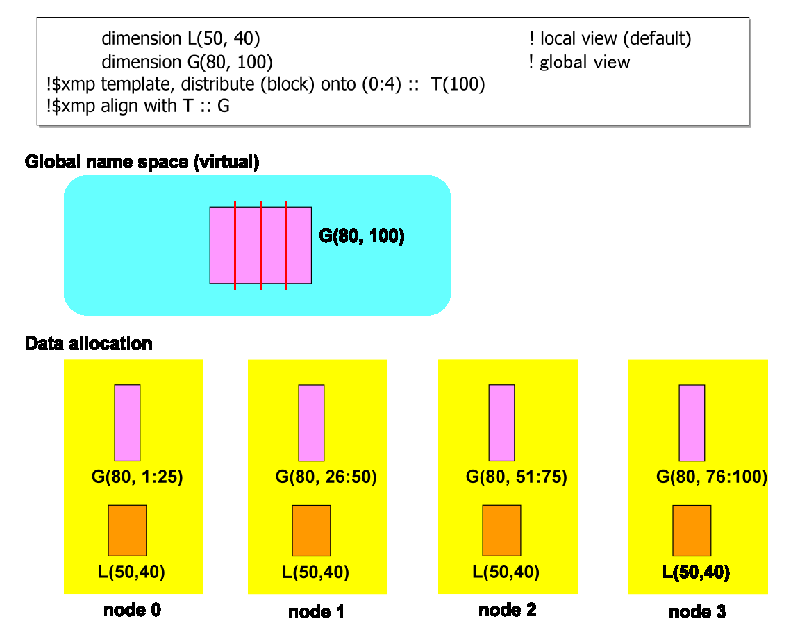
\includegraphics[width=12cm]{figs/Fig4.eps}
  \caption{Global view and local view}
\label{fig4}
\end{myfigure}

\section{Execution model and task}


In \XMP, a program begins as a single thread
of execution in each node. The set of nodes when starting a program is
referred to as the entire node set.

A task is a specific instance of executable
code and its data environment executed in a set of nodes. A task when
starting a program in the entire node set is called an initial task. The
initial task can generate a subtask, which is executed on a subset of the
nodes by the {\tt task} construct. A set of nodes executing the same task is
referred to as the set of executing nodes. If no {\tt task} construct is encountered, then a
program is executed as a single task, and its executing nodes are the entire node set.

If no directives are encountered, then a program is executed
locally. When the same codes are executed, almost the same computation is
performed in each node, which is referred to as duplicate execution. When the threads
encounter a {\tt loop} construct or an {\tt array} construct, the specified
loop is executed in parallel, so that each iteration is assigned to the
node where the specified data element is located. 

A new task is generated by
the {\tt task} construct. A code in the {\tt task} construct is executed
as a subtask executed in a specified node set. When a subroutine is
called in the context of the task, the subroutine is executed on its
executing nodes. 

For synchronization and communication between nodes, a set of
directives is provided. In the local-view programming model, coarray
features are adopted for remote data reference. Note 
that all synchronization and communication are specified explicitly by directives, and without such directives, no communications are
executed implicitly by the compiler.


\section{Glossary}
\subsection*{\Term{node}}
A compute node,
which may have several cores sharing main memory, has its own local
memory. in distributed memory system. Each node is connected via
network. An \XMP program begins as a single thread of execution
in each node.

\subsection*{\Term{node number}}
Unique number assigned to nodes in entire
node. The number starts from 1, larger than or equal to 1 and less
than and equal to the number of nodes. Note that mapping from node
number to MPI rank is decided by the system. The image index of
coarray mapping to the entire nodes is equal to the node number. 

\subsection*{\Term{node set}}
A set of nodes

\subsection*{\Term{entire node set}, \Term{entire node}}
All nodes
executing the program, or a set of the nodes. The entire node set is
decided when staring the program.

\subsection*{\Term{executing node set}, \Term{executing nodes}}
A node set executing a certain region of program. The executing node
set which execute a whole program is a entire node set. The executing
node set of a task is a node set which executes the task. 

\subsection*{\Term{node array}}
A multi-dimensional array containing nodes. Node array have a
name and shape as it attributes.

\subsection*{\Term{executing node array}}
Node array which contain executing node.

\subsection*{\Term{task}}
A specific instance of executable code and
its data environments executed in a set of nodes. In context of
program text, a set of statement executed by a set of nodes. A task
can be nested, and a nested task is executed as a subtask of outer
task.

\subsection*{\Term{template}}
A dummy array used to express an index space associated
with an array. It is also used to describe a iteration space of
loop. Template has a name, dimension and lower and upper bound of each
dimension as attributes.

\subsection*{\Term{replicated execution}}
Execution of the same
code in different nodes. If the state at starting point is same and
the execution has only local side-effect, the local state in each node
remains same. 

\subsection*{\Term{data mapping}}
The combination of alignment and
distribution attributes used to describe how a data object is
allocated to nodes.

\subsection*{\Term{work mapping}}
Assignment of iterations to nodes in
parallel loop, and tasks to nodes.

\subsection*{\Term{image index}}
A number assigned to
each images of coarray. The value is equal to or larger than 1. 
Note that the image index of the coarray mapping to entire nodes is
identical to the node number.

\subsection*{\Term{local}}
Execution of a program has
side-effect only on data in the node. In this case, no communication
to other nodes takes place. 

\subsection*{\Term{non-local}}
Execution of a program requires
communication to other nodes, and has some side-effect to other
nodes. 

\subsection*{\Term{global data}}
Data declared as a distributed array and shared by
nodes.

\subsection*{\Term{local data}}
Data is allocated in each node, and referenced only
within the node.* collective  An operation must be executed by every
node in the executing node set to perform an operation working
together.

\subsection*{\Term{distribution}}
The partition of the index space of a data
object among a set of nodes according to a given pattern. The
{\tt distribute} directive is used to mapping element of a template onto a
set of nodes. 

\subsection*{\Term{alignment}}
An attribute of a data object that establishes
the relationship between data objects for distribution. The {\tt align}
directive is used to describe the correspondence of the element of data
and template. 

\subsection*{\Term{shadow}}
A data area is used to keep neighbor elements
temporarily in distributed array. The shadow is an attribute of
distributed array, declared by {\tt shadow} directive and updated by
{\tt reflect} directive.



\chapter{Directives}\index{directive}

This chapter describes the syntax and behavior of {\XMP} directives.
In this document, the following notation is used to describe {\XMP}
directives. 

\vspace{0.5cm}

\begin{tabular}{ll}
{\tt xxx} & {\tt type-face} characters are used to indicate literal type characters. \\
{\it xxx ...} & If the line is followed by ``...'', then xxx can be
repeated. \\
{\it [xxx]} & {\it xxx} is optional. \\
\verb![F]! & The following lines are effective only in {\Fort}. \\
\verb![C]! & The following lines are effective only in {\C}. \\
\end{tabular}

\vspace{0.5cm}

In {\Fort}, {\XMP} directives are specified using special comments that
are identified by unique sentinels {\tt\verb|!$xmp|}. The rules of
{\Fort} directives in fixed source format and free source format follow
those in {\OMP} and HPF.  In {\C}, {\XMP} directives are specified using
the \verb|#pragma| mechanism provided by the {\C} standards.

\vspace{0.5cm}

\Syntax{directive}
\begin{tabular}{ll}
\verb![F]! & \verb|!$xmp| {\it directive-name clause} \\
& \\
\verb![C]! & \verb|#pragma xmp| {\it directive-name clause} \\
\end{tabular}

\vspace{0.5cm}

Additionally, in {\Fort}, directives of the {\it attribute form}
analogous to type declaration statements in Fortran using the ``{\tt
::}'' punctuation can also be used.

Directives are classified as declarative directives and executable
directives. The declarative directive is a directive that may only be
placed in a declarative context. A declarative directive has no
associated executable user code. The scope rule of declarative
directives obeys that of the declaration statements in the base
language. For example, in C, node declarations by {\tt node} directives
are effective from the declaring point to the end of the function when
specified within a function, or of the file when specified outside any
functions, and, in {\Fort}, node declarations by {\tt node} directives
are effective within the subprogram.

The executable directives are placed in a executable context. A
stand-alone directive is an executable directive that has no associated
user code, such as a {\tt barrier} directive.
%
Some executable directive and its associated user code make up a
directive construct, as in the following format:

\vspace{0.5cm}

\begin{tabular}{ll}
\verb![F]! & \verb|!$xmp| {\it directive-name clause} ...\\
 & \hspace{0.5cm} {\it statement} \\
 & \hspace{0.5cm} ... \\
 & \verb|!$xmp| {\tt end} {\it directive-name} \\
\end{tabular}
\vspace{0.3cm}

Note that in the {\tt loop} construct, {\tt end} can be omitted.

\vspace{0.5cm}

\begin{tabular}{ll}
\verb![F]! & \verb|!$xmp| {\it directive-name clause} ...\\
 & \hspace{0.5cm} {\it do-loop-construct} \\
\end{tabular}

\vspace{0.5cm}

\begin{tabular}{ll}
\verb![C]! & \verb|#pragma xmp| {\it directive-name clause} ...\\
 & \hspace{0.5cm} {\it statement} \\
\end{tabular}

In C, the statement can be a compound-statement.


\section{\Directive{nodes} Directive}

\subsubsection*{Synopsis}

%The {\tt nodes} directive declares a node array with a name, a shape,
%and some attributes.

The {\tt nodes} directive declares a named node array.

\subsubsection*{Syntax}
\Syntax{nodes}

\begin{tabular}{ll}
\verb![F]!&\verb|!$xmp| {\tt nodes} {\it nodes-decl} {\openb},
 {\it nodes-decl} {\closeb}...\\
& \\
\verb![C]!&\verb|#pragma xmp| {\tt nodes} {\it nodes-decl} {\openb},
 {\it nodes-decl} {\closeb}...\\
\end{tabular}

%\begin{tabular}{ll}
%\verb![F]!&\verb|!$xmp| {\tt nodes} {\it nodes-name} \verb|(|
%     {\it nodes-spec} {\openb}, {\it nodes-spec}
%     {\closeb}... \verb|)| \\
%\verb![F]!&\verb|!$xmp| {\tt nodes} {\it nodes-name} \verb|(|
%     {\it nodes-spec} {\openb}, {\it nodes-spec}
%     {\closeb}... \verb|)| {\tt = *}\\
%\verb![F]!&\verb|!$xmp| {\tt nodes} {\it nodes-name} \verb|(|
%     {\it nodes-spec} {\openb}, {\it nodes-spec}
%     {\closeb}... \verb|)| {\tt =} {\it nodes-ref}\\
%& \\
%\verb![C]!&\verb|#pragma xmp| {\tt nodes} {\it nodes-name}
%     \verb|(| {\it nodes-spec} {\openb}, {\it nodes-spec}
%     {\closeb}... \verb|)| \\
%\verb![C]!&\verb|#pragma xmp| {\tt nodes} {\it nodes-name}
%     \verb|(| {\it nodes-spec} {\openb}, {\it nodes-spec}
%     {\closeb}... \verb|)| {\tt = *} \\
%\verb![C]!&\verb|#pragma xmp| {\tt nodes} {\it nodes-name}
%     \verb|(| {\it nodes-spec} {\openb}, {\it nodes-spec}
%     {\closeb}... \verb|)| {\tt =} {\it nodes-ref} \\
%\end{tabular}

\vspace{0.3cm}

where {\it nodes-decl} is one of:

\vspace{0.3cm}

\begin{tabular}{ll}
 \hspace{0.5cm} & {\it nodes-name} \verb|(| {\it nodes-spec} {\openb},
 {\it nodes-spec} {\closeb}... \verb|)| \\
 \hspace{0.5cm} & {\it nodes-name} \verb|(| {\it nodes-spec} {\openb},
     {\it nodes-spec} {\closeb}... \verb|)| {\tt = *} \\
 \hspace{0.5cm} & {\it nodes-name} \verb|(| {\it nodes-spec} {\openb},
     {\it nodes-spec} {\closeb}... \verb|)| {\tt =} {\it nodes-ref} \\
\end{tabular}

\vspace{0.3cm}

and {\it nodes-spec} must be one of:

\vspace{0.3cm}

\begin{tabular}{ll}
 \hspace{0.5cm} & {\it int-expr} \\
 \hspace{0.5cm} & {\tt *} \\
\end{tabular}


\subsubsection*{Description}

The {\tt nodes} directive declares a node array that corresponds to a
node set.

The first form of the {\tt nodes} directive is used to declare a node
array that corresponds to the entire node set.
%The second and third forms declare a new node array with a name, a
%dimension, and a size in order to reference a set of nodes.
The second form is used to declare a node array that corresponds to the
executing node set.
%The ``{\tt *}'' symbol specifies the current executing node set.
The third form is used to declare a node array that corresponds to the
node set specified by {\it nodes-ref}.

%If {\it map-type} is specified as {\tt regular}, then the order of nodes in
%the node array follows that of the {\Fort} array. Therefore, in the first
%form, the node number is used to order nodes in the node array with
%{\Fort} array ordering. In the second and third forms, the nodes are
%ordered according to the sequence association with referenced nodes.  
%
%If no {\it map-type} is specified, then the ordering nodes in the node array are
%system dependent. It is desirable to order the nodes in order to make use of
%the network topology for efficient communication. 

If {\it node-size} in the last dimension is ``{\tt *}'', then the size
of the node array is automatically adjusted according to the total size
of the entire node set in the first form, the executing node set in the
second form, or the referenced node set in the third form.

\subsubsection*{Restrictions}

\begin{itemize}
%\item {\it nodes-name} is an identifier in class (1) and must not
%  conflict with other names in class (1).
\item {\it nodes-name} must not conflict with any other local name in
      the same scoping unit.
%\item \verb![F]! The second form cannot be used in either the main
%      program or a module.
\item {\it nodes-spec} can be ``{\tt *}'' only in the last dimension.
\item {\it nodes-ref} must not reference {\it nodes-name} either
      directly or indirectly.
\item If no {\it nodes-spec} is ``{\tt *}'', then the product
      of all {\it nodes-spec} must be equal to the total size of the
      entire node set in the first form, the executing node set in the
      second form, or the referenced node set in the third form.
%
%      The referenced node set must consist of all nodes in the first form,
%      the executing node set in the second form, and the node set
%      referenced by {\it nodes-ref} in the third form. 
\item {\it nodes-subscript} in {\it nodes-ref} must not be ``{\tt *}''.
\end{itemize}

\subsubsection*{Examples}
\Example{nodes}

The following are examples of the first and the third forms appeared in
the main program. Since the node array {\tt p}, which corresponds to the
entire node set, is declared to be of size 16, this program must be
executed by 16 nodes.

%Since the declaration of node array {\tt p} specifies
%16 nodes as its size, this program must be executed with 16 nodes.

%Since {\tt regular} is not specified, it is not guaranteed that {\tt
%Ar(1)} and {\tt p(3)} are the same node, and the node number of {\tt
%z(1,1)} is 1.

\vspace{0.5cm}

\begin{minipage}{0.45\hsize}
\begin{center}
\begin{XFexample}
      program main
!$xmp nodes p(16)
!$xmp nodes q(4,*)
!$xmp nodes r(8)=p(3:10)
!$xmp nodes z(2,3)=(1:6)
      ...       
      end program 
\end{XFexample}
\end{center}
\end{minipage}
%
\begin{minipage}{0.45\hsize}
\begin{center}
\begin{XCexampleR}
int main() {
#pragma xmp nodes p(16)
#pragma xmp nodes q(4,*)
#pragma xmp nodes r(8)=p(3:10)
#pragma xmp nodes z(2,3)=(1:6)
    ...
}
\end{XCexampleR}
\end{center}
\end{minipage}

\vspace{0.5cm}

%Example using the regular option. Since node array {\tt p} is declared
%without the regular option, it is not guaranteed that {\tt p(1), p(2)}
%have the node number 1, 2, ... and so on. The node array {\tt q} with the 
%regular option has the order in which
%{\tt q(1,1), q(2,1), q(3,1), q(4,1), q(1,2), ...} have node numbers
%1,2,3,4,5, ... In node array z with the regular option,
%{\tt z(1,1), z(2,1), z(1,2), z(2,2), z(1,3), z(2,3), ...} have the
%node numbers 1, 2, 3, 4, 5, 6, ...
%
%\begin{XFexample}
%      program main
%!$xmp nodes p(16)
%!$xmp nodes(regular) q(4,*)
%!$xmp nodes(regular) r(8)=p(3:10)
%!$xmp nodes(regular) z(2,3)=(1:6)
%      ...
%      end program
%\end{XFexample}

The following is an example of a node declaration in a procedure.
Since {\tt p} is declared in the second form to be of size 16 and
corresponds to the executing node set, the invocation of the {\tt foo}
function must be executed by 16 nodes.
%
The node array {\tt q} is declared in the first form and corresponds to
the entire node set. The node array {\tt r} is declared as a subset of
{\tt p}, and {\tt x} as a subset of {\tt q}.

%The declaration for the node array {\tt q} of the first form
%declares the node array for the entire node set. The node array {\tt r}
%is a subset of {\tt p}, and the node array of {\tt x} is a subset of
%{\tt q}.

\begin{XFexample}
      function foo()
!$xmp nodes p(16)=*
!$xmp nodes q(4,*)
!$xmp nodes r(8)=p(3:10)
!$xmp nodes x(2,3)=q(1:2,1:3)
      ...
      end function
\end{XFexample}


\subsection{Node Reference}

\subsubsection*{Synopsis}

The \Term{node reference} expression is used to reference a subset of a
node set.

\subsubsection*{Syntax}
\index{node reference}
\index{Syntax!{node reference}}

A node reference {\it nodes-ref} is specified by either node number
or the name of a node array.

\begin{center}
\begin{tabular}{lll}
{\it nodes-ref} & {\bf is} & \verb|(| {\it nodes-subscript} \verb|)|\\ 
                & {\bf or} & {\it nodes-name} {\openb}\verb|(| {\it nodes-subscript}
	 {\openb}, {\it nodes-subscript} {\closeb}... \verb|)|{\closeb} \\
\end{tabular}
\end{center}
%
\vspace{0.3cm}
%
where {\it nodes-subscript} must be one of:

\hspace{\hsize}

\begin{tabular}{ll}
 \hspace{0.5cm} & {\it int-expr} \\
 \hspace{0.5cm} & {\it triplet} \\
 \hspace{0.5cm} & {\tt *} \\
\end{tabular}

%\begin{center}
%\begin{tabular}{ll}
%{\it nodes-ref} & {\it node-number-ref} $\vert$ {\it named-nodes-ref} \\
%{\it node-number-ref} & {\it node-number} $\vert$ ([{\it
%     node-number}]:[{\it node-number}][:{\it int-expr}]) \\
%& {\it node-number} is a positive number. \\
%{\it named-nodes-ref} & {\it nodes-name} [ ( {\it nodes-subscript}
%[,  ...] ) ] \\
%{\it nodes-subscript} & {\it int-expr} $\vert$ {\it triplet} $\vert$ {\tt *} \\
%\end{tabular}
%\end{center}

\subsubsection*{Description}

Node reference by node number represents a node set specified by a
node number of the entire node set or a triplet describing a set of node
numbers of the entire node set.

Node reference by name represents a node set specified by the name of a
node array or its subarray.

%The subscript of the subarray of a node array must be either an integer,
%a triplet, or ``{\tt *}''. The notation of the subarray using a triplet
%in the subscript is the same as that in {\Fort}. 

Specifically, the ``{\tt *}'' symbol appeared as {\it nodes-subscript}
in a dimension of {\it nodes-ref} is interpreted by each node at runtime
as its position (coordinate) in the dimension of the referenced node
array.
%The ``{\tt *}'' symbol in {\it nodes-subscript} in a subarray of a
%node array specifies a subscript associated with the executing node in
%the node array of the executing node set.
%
Thus, a node reference {\tt p($s_1$, ..., $s_{k-1}$, *, $s_{k+1}$, ...,
$s_n$)} is interpreted as {\tt p($s_1$, ..., $s_{k-1}$, $j_k$,
$s_{k+1}$, ..., $s_n$)} on the node {\tt p($j_1$, ..., $j_{k-1}$, $j_k$,
$j_{k+1}$, ..., $j_n$)}.

%Thus, the following node is referenced by name with the $k$-th subscript
%``{\tt *}'':
%
%\begin{center}
%{\tt p($s_1$, ..., $s_{k-1}$, *, $s_{k+1}$, ..., $s_n$)} 
%\end{center}
%where, with the exception of $s_k$, subscripts $s_i$ must not be ``{\tt *}'', 
%is evaluated at the node 
%\begin{center}
%{\tt p($j_1$, ..., $j_{k-1}$, $j_k$, $j_{k+1}$, ..., $j_n$)} 
%\end{center}
%where $j_i$ is an integer, in
%\begin{center}
%{\tt p($s_1$, ..., $s_{k-1}$, $j_k$, $s_{k+1}$, ..., $s_n$)}.
%\end{center}

Note that ``{\tt *}'' can be used only as the node reference in
the {\tt on} clause of some executable directives.

%This node reference composes the node set using nodes with the $k$-th
%subscript $j_k$. The same rule is applied even if more than two
%subscripts are ``{\tt *}''. This notation can be used only in the node
%reference of the on clause in executable directives. 

\subsubsection*{Examples}
\index{node reference}
\index{Example!{node reference}}

Assume that {\tt p} is the name of a node array and that {\tt m} is an
integer variable.

\begin{itemize}
\item As a target node array in the {\tt distribute} directive,

\Example{distribute}
\begin{tabular}{l}
\verb|!$xmp distribute a(block) onto p| \\
\end{tabular}%$

\item To specify a node set to which the declared node array corresponds
      in the second form of the {\tt nodes} directive,

\Example{nodes}
\begin{tabular}{l}
\verb|!$xmp nodes r(2,2,4) = p(1:4,1:4)| \\
\verb|!$xmp nodes r(2,2,4) = (1:16)| \\
\end{tabular}

\item To specify a node array that corresponds to the executing node set
      of a task in the {\tt task} directive,

\Example{task}
\begin{tabular}{l}
\verb|!$xmp task on p(1:4,1:4)| \\
\verb|!$xmp task on (1:16)| \\
\verb|!$xmp task on p(:,*)| \\
\verb|!$xmp task on (m)| \\
\end{tabular}

\item To specify a node array with which iterations of a loop are
      aligned in the {\tt loop} directive,

%In the {\tt loop} directive, sets of executing nodes are specified
%      for the iterations.

\Example{loop}
\begin{tabular}{l}
\verb|!$xmp loop (i) on p(lb(i):lb(i+1)-1)| \\
\end{tabular}%$

\item To specify a node array that corresponds to the executing node set
      in the {\tt barrier} and the {\tt reduction} directive,

%In {\tt barrier} directive and the {\tt reduction} directive,
%executing nodes are specified. 

\Example{barrier}
\Example{reduction}
\begin{tabular}{l}
\verb|!$xmp barrier on p(5:8)| \\
\verb|!$xmp reduction (+:a) on p(*,:)| \\
\end{tabular}

\item To specify the source node and the node array that corresponds to
      the executing node set in the {\tt bcast} directive,

%In the {\tt bcast} directive, a source node and executing nodes are specified.

\Example{bcast}
\begin{tabular}{l}
\verb|!$xmp bcast (b) from p(k) on p(:)| \\
\end{tabular}
\end{itemize}

%\subsubsection*{Examples}
%\Example{nodes}
%\Example{tasks}
%\Example{task}
%\Example{end task}
%\Example{end tasks}
%
%\begin{minipage}{0.45\hsize}
%\begin{center}
%\begin{XFexample}
%      subroutine caller
%!$xmp nodes p(1000)
%      real a(100,100)
%      ...
%!$xmp tasks
%!$xmp  task on p(1:500)
%        call task1(a)
%!$xmp  end task
%!$xmp  task on p(501:800)
%        call task1(a)
%!$xmp  end task
%!$xmp  task on p(801:1000)
%        call task1(a)
%!$xmp  end task
%!$xmp end tasks
%      ...
%      end do
%\end{XFexample}
%\end{center}
%\end{minipage}
%\begin{minipage}{0.45\hsize}
%\begin{center}
%\begin{XFexampleR}
%      subroutine task1(a)
%      ...
%!$xmp nodes q(*)
%      real a(100,100)
%      ...
%      end subroutine
%\end{XFexampleR}
%\end{center}
%\end{minipage}
%\vspace{1cm}


\subsection{Correspondence between Node Arrays}

If one node array and the other have the same shape and correspond to
the same node set, an element of the one and an element of the other are
assigned to the same node;
%
otherwise, correspondence between any two node arrays is not specified.

\section{Template and data mapping}

\subsection{Template directive}
\subsubsection*{Synopsis}

The {\tt \Directive{template}} directive declares a template. 

\subsubsection*{Syntax}
\Syntax{template}

\begin{tabular}{ll}
\verb![F]! & \verb|!$xmp| {\it template-name} ( {\it template-spec} 
[, {\it template-spec} ] ... ) \\
& \\
\verb![C]! & \verb|#pragma xmp|  {\it template-name} ( {\it template-spec} 
[, {\it template-spec} ] ... ) \\
\end{tabular}
\vspace{0.3cm}

where {\it template-spec} must be one of:

\hspace{\hsize}

\begin{tabular}{ll}
 \hspace{0.5cm} & [{\it int-expr} {\tt :}] {\it int-expr} \\
 \hspace{0.5cm} & {\tt :} \\
\end{tabular}

\subsubsection*{Description}

The {\tt template} directive declares a template with the shape specified by
the sequence of {\it template-spec}. If all expressions in the sequence of
{\it template-spec} are �e�e:", then the shape of the template is initially
undefined. This template must not be referenced until the shape is
defined by {\it template\_fix} directives at run-time. If {\it
  int-expr} is specified as {\it template-spec}, then the default lower bound
is 1. 

\subsubsection*{Restrictions}

\begin{itemize}
\item Each {\it template-spec} must be either all [{\it int-expr} {\tt :}] {\it
  int-expr}
 or all �e�e:".
\end{itemize}

\subsection{Template reference}

\subsubsection*{Synopsis}

The template reference expression is
used to reference a subset of the referenced template.

\subsubsection*{Syntax}
\Syntax{template reference}

\begin{center}
\begin{tabular}{ll}
{\it template-ref} & {\it template-name} [ ( {\it template-subscript}
[,  ...] ) ] \\
{\it template-subscript} & {\it int-expr} | {\it triplet} | {\tt *} \\
\end{tabular}
\end{center}

\subsubsection*{Description}

The template reference refers to a subarray of the template array.  

The subscript
of the subarray of a template array must be either an integer, a triplet, or
�e�e{\tt *}". The notation of the subarray using a triplet in the subscript is the same as
that in \Fort. 

\subsubsection*{Examples}

Assume that {\tt t} is a template name. 

\begin{itemize}
\item In the {\tt task} directive, a set of executing nodes is indirectly specified for the task.

\Example{task}
\begin{tabular}{l}
\verb|!$xmp task on t(1:m,1:n)| \\
\verb|!$xmp task on t| \\
\end{tabular}

\item In the {\tt loop} directive, an element of the template at which each loop iteration is aligned.

\Example{loop}
\begin{tabular}{l}
\verb|!$xmp loop (i) on t(i-1)| \\
\end{tabular}

\item In the {\tt array} directive, a template which the following array assignment statement is aligned with. 

\Example{array}
\begin{tabular}{l}
\verb|!$xmp array on t(1:n)| \\
\end{tabular}

\item In the {\tt barrier}, {\tt reduction}, and {\tt bcast} directives,
executing nodes are specified indirectly. 

\Example{barrier}
\Example{reduction}
\begin{tabular}{l}
\verb|!$xmp barrier on t(1:n)| \\
\verb|!$xmp reduction (+:a) on t(*,:)| \\
\verb|!$xmp bcast b from p(k) on t(1:n)| \\
\end{tabular}

\end{itemize}

\subsection{Distribute directive}

\subsubsection*{Synopsis}
The {\tt \Directive{distribute}} directive specifies a distribution of templates. 

\subsubsection*{Syntax}
\Syntax{distribute}

\begin{tabular}{ll}
\verb![F]! & \verb|!$xmp| {\tt distribute}{\it template-name} 
({\it dist-format}[,{\it dist-format}]... ) {\tt onto} {\it nodes-name} \\
& \\
\verb![C]! & \verb|#pragma xmp| {\tt distribute}{\it template-name} 
({\it dist-format}[,{\it dist-format}]... ) {\tt onto} {\it nodes-name} \\
\end{tabular}
\vspace{0.3cm}

where {\it dist-format} must be one of:

\begin{tabular}{ll}
 \hspace{0.5cm} & {\tt *} \\
 & {\tt block} \\
 & {\tt cyclic} [ ( {\it int-expr} ) ] \\
 & {\tt gblock} ( {\tt *} $\vert$ {\it int-array} ) \\
\end{tabular}

\subsubsection*{Description}

According to the specified
distribution format, a template is distributed onto a set of nodes. The
dimension of the node set appearing in an {\tt onto} clause corresponds, in
left-to-right order, with the dimension of the distributed template for
which the corresponding dist-format is not �e�e*". 

The interpretation of dist-format is as follows:

\begin{description}
\item[{\tt *}]
The corresponding dimension is not distributed.

\item[{\tt block}]
The corresponding dimension of the template is
divided into contiguous blocks of the same size, which are distributed
onto the corresponding dimension of the node set. Let {\tt d} be the size of
the corresponding dimension of the template, and let {\tt p}be  the size of the
corresponding dimension of node sets. If {\tt d mod p} is not zero, then the
dimension of the template is divided into {\tt d/ceil(d/p)} blocks of size
{\tt ceil(d/p)} and one block of size {\tt d\%ceil(d/p)}, and each
block is assigned sequentially to an index along the corresponding
dimension of the node set. Note that
if {\tt k=p-d/ceil(d/p)-1 > 0}, then there is no block for the last
{\tt k} indices.

\item[{\tt cyclic}]
Equivalent to {\tt cyclic(1)}.

\item[{\tt cyclic(n)}]
The corresponding
dimension of the template is divided into contiguous blocks of 
size {\tt n}, and these blocks are distributed onto the corresponding
dimension of the node set in a round-robin manner.

\item[{\tt gblock(m)}]
{\tt m} is a mapping array. The corresponding dimension of the template is
divided into contiguous blocks so that the ith block is of size
{\tt m(i)}, and these blocks are 
distributed onto the corresponding dimension of the node set.
\end{description}

If more than one {\tt gblock(*)} is specified in {\it
  dist-format}, then the template must not be referenced until the shape of
the template is defined by {\it template\_fix} directives at run-time. 


\subsubsection*{Restrictions}

\begin{itemize}
\item The number of {\it dist-format}, which is not �e�e*", must be equal to the
  rank of the node set specified by {\it nodes-name}.  
\item The array {\it int-array} in parentheses following {\tt gblock}
  must be an integer one-dimensional array, and its size must be equal
  to the size of the corresponding dimension of the node set.
\item The element of the {\it int-array} array in 
parentheses following {\tt gblock} must be a non-negative integer.
\item The sum of the elements of the {\it int-array} array in parentheses
  following {\tt gblock} must be equal to or greater than the size of the
  corresponding dimension of the template specified by {\it template-name}.
\end{itemize}

\subsubsection*{Examples}
\Example{nodes}
\Example{template}
\Example{distribute}

\begin{description}
\item[Example 1]
\hspace{\hsize}
\begin{Fexample}
      program main
!$xmp nodes p(8,5)
!$xmp template t(64,64,64)
!$xmp distribute t(*,cyclic,block) onto p
\end{Fexample}

The template {\tt t} is distributed in block format, as
shown in the following:

\begin{center}
\begin{tabular}{|c|c|}
\hline
{\tt p(1)} & {\tt t(1:16)} \\
\hline
{\tt p(2)} & {\tt t(17:32)} \\
\hline
{\tt p(3)} & {\tt t(33:48)} \\
\hline
{\tt p(4)} & {\tt t(49:64)} \\
\hline
\end{tabular}
\end{center}

\item[Example 2]
\hspace{\hsize}
\begin{Fexample}
      program main
!$xmp nodes p(4)
!$xmp template t(64)
!$xmp distribute t(cyclic(8)) onto p
\end{Fexample}

The template {\tt t} is distributed in a cyclic format of size eight, as
shown in the following:

\begin{center}
\begin{tabular}{|c|c|}
\hline
{\tt p(1)} & {\tt t(1:8) t(33:40)} \\
\hline
{\tt p(2)} & {\tt t(9,16) t(41:48)} \\
\hline
{\tt p(3)} & {\tt t(17,24) t(49:56)} \\
\hline
{\tt p(4)} & {\tt t(25,32) t(57:64)} \\
\hline
\end{tabular}
\end{center}

\item[Example 3]
\hspace{\hsize}
\begin{Fexample}
      program main
!$xmp nodes p(8,5)
!$xmp template t(64,64,64)
!$xmp distribute t(*,cyclic,block) onto p
\end{Fexample}

The first dimension of template
{\tt t} is not distributed. The second dimension is distributed onto the
first dimension of node set {\tt p} in cyclic format. The third
dimension is distributed onto the second dimension of node set {\tt p}
in block format. The results are as follows: 

\begin{center}
\begin{tabular}{|c|c|}
\hline
{\tt p(1)} & {\tt t(1:64, 1:57:8, 1:13)} \\
\hline
{\tt p(2)} & {\tt t(1:64, 2:58:8, 1:13)} \\
\hline
... & ... \\
\hline
{\tt p(4)} & {\tt t(1:64), 8:64:8, 53:64)} \\
\hline
\end{tabular}
\end{center}

where the size of the third dimension is 64 and is not divisible by the
size of the second dimension of {\tt p}. Then, the sizes of a number of blocks in the third
dimension are different. 

\end{description}

\subsection{Align directive}
\subsubsection*{Synopsis}
The {\tt \Directive{align}} directive specifies that arrays are to be mapped in
the manner given by a template.

\subsubsection*{Syntax}
\Syntax{align}

\begin{tabular}{ll}
\verb![F]! & \verb|!$xmp| {\tt align} {\it array-name}
( {\it align-source} [, {\it align-source}] ... ) \\
 & {\tt with} {\it template-name}
({\it align-subscript} [, {\it align-subscript}] ... ) \\
& \\
\verb![C]! & \verb|#pragma xmp| {\tt align} {\it array-name} 
{\tt [}{\it align-source}{\tt ]} [{\tt [}{\it align-source}{\tt ]}] ... \\
 & {\tt with} {\it template-name}
({\it align-subscript} [, {\it align-subscript}] ... ) \\
\end{tabular}
\vspace{0.3cm}

where {\it align-source} must be one of:

\begin{tabular}{ll}
 \hspace{0.5cm} & {\tt scalar-int-variable} \\
 & {\tt *} \\
 & {\tt :} \\
\end{tabular}
\vspace{0.3cm}

and {\tt align-subscript} must be one of:

\begin{tabular}{ll}
 \hspace{0.5cm} & {\tt scalar-int-variable} [ ( {\tt +} $\vert$ {\tt -} )
 {\it int-expr} ] \\
 & {\tt *} \\
 & {\tt :} \\
\end{tabular}
\vspace{0.3cm}

Note that the variable {\it scalar-int-variable} appearing in {\it
  align-source} is referred to as a �e�e\Term{align dummy variable}". 

\subsubsection*{Description}
The array specified by {\it array-name} is
aligned with the template specified by {\it template-name}. Each element
indexed by the sequence of {\it align-source} is aligned with the element of
the template indexed by the sequence of {\it align-subscript}, where {\it align-source} and {\it align-subscript} are interpreted as follows:  

\begin{enumerate}
\item The first form of
{\it align-source} and {\it align-subscript} describes an align dummy variable and its (restricted) expression, respectively. The range of the align dummy
variable covers all valid index values in the corresponding
dimension of the array.
\item The second form �e�e*" of {\it align-source} and {\it
    align-subscript} describes a dummy variable (not an align dummy
  variable) that does not appear anywhere in the directive.
\begin{itemize} 
\item The second form of the align-source is said to �e�ecollapse"
the corresponding dimension of the array. As a result, the index along the
corresponding dimension makes no difference in determining the alignment.
\item The second form of the align-subscript is said to �e�ereplicate"
the array. Each element of the array is replicated and aligned to
all index values in the corresponding dimension of the template.
\end{itemize}
\item Both {\it align-source} and {\it align-subscript} are �e�e:",
  then each element of an array 
is aligned with each element of the template.
\end{enumerate}

\subsubsection*{Restrictions}

\begin{itemize}
\item In the sequence of {\it align-subscript}, the same align variable must not appear more than once. 
\item  In {\it align-subscript}, an align dummy variable must not appear more than once. 
\item  In {\it int-expr} of {\it align-subscript}, an align dummy variable must not appear.
\item  If either {\it align-source} or {\it align-subscript} is
  �e�e:", then the corresponding {\it align-source} or 
{\it align-subscript} must be �e�e:". 
\end{itemize}

\subsubsection*{Examples}
\Example{align}

\begin{description}
\item[Example 1]
\hspace{\hsize}
\begin{Fexample}
!$xmp align a(i) with t(i)
\end{Fexample}

The array element {\tt a(i)} is aligned with  the template element {\tt
  t(i)}. This is equivalent to the following:

\begin{Fexample}
!$xmp align a(:) with t(:)
\end{Fexample}

\item[Example 2]
\hspace{\hsize}
\begin{Fexample}
!$xmp align a(*,j) with t(j)
\end{Fexample}

The subarray {\tt a(:,j)} is aligned with the template
element {\tt (j)}. Note that the first dimension of {\tt a} is collapsed.

\item[Example 3]
\hspace{\hsize}
\begin{Fexample}
!$xmp align a(j) with t(*,j)
\end{Fexample}

The array element {\tt a(j)} is replicated and aligned with each
template element {\tt t(1,j) $\sim $ t(10,j)}. Assume that the upper and
lower bounds of the first dimension of the template {\tt t} are 1 and 10, respectively.

\item[Example 4]
\hspace{\hsize}
\begin{Fexample}
!$xmp template t(n1,n2)
      real a(m1,m2)
!$xmp align a(*,j) with t(*,j)
\end{Fexample}

The subarray {\tt a(:,j)} is aligned with each template
element, {\tt t(1,j) $\sim $ t(n1,j)}. 

If �e�e*" in the first dimension of array {\tt a} is replaced by dummy
variable {\tt i}, and �e�e*" in the first dimension of the template is
replaced by dummy variable {\tt k}, then we have:

$${a(i,j) \rightarrow t(k,j) | (i,j,k) \in (1:n1,1:n2,1:m1)}$$

\end{description}

\subsection{Shadow directive}
\subsubsection*{Synopsis}

The {\tt \Directive{shadow}} directive declares and allocates a shadow area for a
distributed array.

\subsubsection*{Syntax}
\Syntax{shadow}

\begin{tabular}{ll}
\verb![F]! & \verb|!$xmp| {\tt shadow} {\it array-name}
( {\it shadow-width} [, {\it shadow-width}] ... ) \\
& \\
\verb![C]! & \verb|#pragma xmp|  {\tt shadow} {\it array-name}
{\tt [}{\it shadow-width}{\tt ]} [{\tt [}{\it shadow-width}{\tt ]}] ... \\
\end{tabular}
\vspace{0.3cm}

where {\it shadow-width} must be one of:

\begin{tabular}{ll}
 \hspace{0.5cm} & {\it int-expr} \\
 & {\it int-expr} : {\it int-expr}\\
 & \verb|*|\\
\end{tabular}

\subsubsection*{Description}

The {\tt shadow} directive specifies the shadow width for which the area is used to communicate the neighbor element of the block of an array specified by {\it array-name}, which is distributed
onto each node. When {\it shadow-width} is of the form 
{\it int-expr} : {\it int-expr}, the shadow area is added at the upper and
lower bounds with the width specified in the specified dimension. When
{\it shadow-width} is a form of {\it int-expr}, the shadow area is added at the upper
and lower bounds with the same width specified in the specified
dimension. When shadow-width is of the form �e�e\verb|*|", the entire area of the
array is allocated on each node, and all of the area that it does not own
is regarded as shadow. Note that this type of shadow is sometimes referred to as a �e�efull shadow."

The data stored in the storage area declared by the {\tt shadow} directive is referred to as a
\Term{shadow object}. The shadow object can be explicitly defined and referenced
only by the method described below. Of the data allocated to a storage
area other than a shadow area, data representing the same array
element as that of a shadow object is referred to as a reflection source of
the shadow object. Conceptually, a shadow object and its reflection
source are not mapped to the same processor at the same time.
%A shadow
%object is not mapped to a processor to which its reflection source is
%mapped. 

\subsubsection*{Restrictions}

\begin{itemize}
\item The value specified by {\it shadow-width} must be a
non-negative integer. 
\end{itemize}

\subsection{\Directive{template\_fix} directive}
\subsubsection*{Synopsis}
This directive is an executable directive that fixes the shape of the template. 

\subsubsection*{Syntax}
\Syntax{template\_fix}

%\begin{tabular}{ll}
%\verb![F]! & \verb|!$xmp| {\tt template\_fix} {\it template-name} \\
% & [({\it template-spec} [, {\it template-spec}] ... )] \\
% & [, {\tt distribute} ( {\it dist-format} [, {\it dist-format}]... ) \\
%& \\
%\verb![C]! & \verb|#pragma xmp|  {\tt template\_fix} {\it template-name} \\
% & [({\it template-spec} [, {\it template-spec}] ... )] \\
% & [, {\tt distribute} ( {\it dist-format} [, {\it dist-format}] ...) \\
%\end{tabular}
\begin{tabular}{ll}
\verb![F]! & \verb|!$xmp| {\tt template\_fix} ( {\it dist-format} [,
 {\it dist-format}]... )\\
 & {\it template-name} [({\it template-spec} [, {\it template-spec}] ... )] \\
& \\
\verb![C]! & \verb|#pragma xmp|  {\tt template\_fix} ( {\it dist-format}
     [, {\it dist-format}] ...)\\
 & {\it template-name} [({\it template-spec} [, {\it template-spec}] ... )] \\
\end{tabular}
\vspace{0.3cm}

where {\it template-spec} is:

\begin{tabular}{ll}
 \hspace{0.5cm} & [{\it int-expr} :] {\it int-expr} \\
\end{tabular}
\vspace{0.3cm}

where {\it dist-format} is one of:

\begin{tabular}{ll}
 \hspace{0.5cm} & {\tt *} \\
 & {\tt block} \\
 & {\tt cyclic} [( {\it int-expr} )] \\
 & {\tt gblock} ( {\it int-array} ) \\
\end{tabular}

\subsubsection*{Description}

The {\tt template\_fix} directive is an executable directive to fix the
shape of the template, which is initially undefined, by specifying the
sizes of each dimension and the distribution format at run-time. The array
aligned to an initially undefined template must be an allocatable
array, which cannot be allocated until the template is fixed by the
{\tt template\_fix} directive. Any executable directives that have such a
template in their {\tt on} clause must not be executed before the
template is fixed by the
{\tt template\_fix} directive. Any undefined template can be fixed only
once by the {\tt template\_fix} directive. 

Note that the meaning of
{\it dist-format} in the {\tt distribute} clause is the same as that in
the {\tt distribute} directive.

\subsubsection*{Restrictions}
\begin{itemize}
\item When the {\tt template\_fix} directive is executed, the
template specified by template-name must be undefined.
\item The sequence
of {\it dist-format} in the {\tt template\_fix} directive and the sequence
of {\it dist-format} in the {\tt distribute} directive specified by
{\it template-name} must be identical, except for the brackets following {\tt
  gblock}. 
\item The sequence of either the {\it template-spec} or {\tt distribute}
  clause must be given. 
\item The {\tt template\_fix} directive must appear in executable context.
\end{itemize}

\subsubsection*{Example}
\Example{template}
\Example{distribute}
\Example{align}
\Example{template\_fix}

\begin{Fexample}
!$xmp template :: t(:)
!$xmp distribute (gblock(*)) :: t

      real , allocatable :: a(:)
!$xmp align (i) with t(i) :: a
      ...
      N = ...; M(...) = ...
      ...
!$xmp template_fix(gblock(M)) t(N)
      ...
      allocate (a(N))
\end{Fexample}

Since the shape is {\tt (:)} and the distribution format is {\tt gblock(*)},
the template {\tt t} is initially undefined. The allocatable array
{\tt a} is aligned to {\tt t}. After the size {\tt N} of {\tt t} and the mapping array {\tt M} is defined, {\tt t} is fixed by the {\tt template\_fix} directive, and {\tt a} is allocated.

\section{Work mapping construct}

\subsection{{\tt task} construct}

\subsubsection*{Synopsis}

The {\tt \Directive{task}} construct defines a task that is executed by
a specified node set.

\subsubsection*{Syntax}
\Syntax{task}

\begin{tabular}{ll}
\verb![F]! & \verb|!$xmp| {\tt task on} \{{\it nodes-ref} $\vert$ {\it
 template-ref}\} \\
& {\it block} \\
& \verb|!$xmp| {\tt end task} \\
& \\
\verb![C]! & \verb|#pragma xmp| {\tt task on} \{{\it nodes-ref} $\vert$
     {\it template-ref}\} \\
& {\it block} \\
\end{tabular}

\subsubsection*{Description}

When a node encounters a {\tt task} construct at runtime, it executes
the associated block (called a {\it task}) if it is included by the node
set specified by the {\tt on} clause; otherwise it skips executing the
block.

%This line was inserted by Sakagami for svn test. 

Unless a task is surrounded by a {\tt \Directive{tasks}} construct,
{\it nodes-ref} or {\it template-ref} in the {\tt on} clause is
evaluated at the entry of the task; otherwise {\it nodes-ref} and {\it
template-ref} of the {\tt task} construct are evaluated at the entry of
the surrounding {\tt tasks} construct, where the evaluation results must
be the same in every node in the executing node set.

When {\it nodes-ref} or {\it template-ref} is evaluated, the
corresponding new executing node set is created conceptually. The former
executing node set that includes the node encountering the {\tt task}
construct is referred to as the ``\Term{parent executing node set}'' of
the new executing node set.

\subsubsection*{Restrictions}

\begin{itemize}
\item The node set specified by {\it nodes-ref} or {\it template-ref}
      in the {\tt on} clause of a {\tt task} construct must be a subset
      of the parent executing node set.
\end{itemize}


\subsection{{\tt tasks} construct}

\subsubsection*{Synopsis}

The {\tt \Directive{tasks}} construct is used to instruct nodes in
the executing node set to execute the multiple tasks it surrounds in
arbitray order.

\subsubsection*{Syntax}
\Syntax{tasks}

\begin{tabular}{ll}
\verb![F]! & \verb|!$xmp| {\tt tasks} {\openb} {\tt nowait} {\closeb} \\
& {\it task-construct} \\
& ... \\
& \verb|!$xmp| {\tt end tasks} \\
& \\
\verb![C]! & \verb|#pragma xmp| {\tt tasks} {\openb} {\tt nowait} {\closeb} \\
& {\tt \{} \\
& \hspace{0.5cm} {\it task-construct} \\
& \hspace{0.5cm} ... \\
& {\tt \}} \\
\end{tabular}

\subsubsection*{Description}

{\tt \Directive{task}} constructs (called {\it child tasks}) surrounded
by a {\tt tasks} construct are executed in arbitrary order without
implicit synchronization at the entry of each child task.
%
As a result, if there is no overlap between the executing node sets of
the adjacent child tasks, they can be executed in parallel.

Conceptually, {\it nodes-ref} or {\it template-ref} in the {\tt task}
constructs of child tasks are evaluated at the entry of their
surrounding {\tt tasks} construct.

No implicit synchronization is performed at the entry of the {\tt tasks}
construct;
%
implicit synchronization is performed at the exit of the {\tt tasks}
construct, which guarantees that all communications issued inside child
tasks are completed, unless a {\tt nowait} clause is specified.

%When a {\tt nowait} clause is specified, implicit
%synchronization is not performed at the end of the {\tt tasks}
%construct. Without a {\tt nowait} clause, implicit synchronization is
%performed in order to gurantee that all communications issued inside
%child tasks are completed.

\subsubsection*{Example}
\Example{tasks}
\Example{task}
\Example{end tasks}
\Example{end task}

\begin{minipage}{0.45\hsize}
\begin{center}
\begin{Fexample}
      subroutine caller
!$xmp nodes p(1000)
      real a(100,100)
      ...
!$xmp tasks
!$xmp  task on p(1:500)
        call task1(a)
!$xmp  end task
!$xmp  task on p(501:800)
        call task1(a)
!$xmp  end task
!$xmp  task on p(801:1000)
        call task1(a)
!$xmp  end task
!$xmp end tasks
      ...
      end do
\end{Fexample}
\end{center}
\end{minipage}
%
\begin{minipage}{0.45\hsize}
\begin{center}
\begin{FexampleR}
      subroutine task1(a)
      ...
!$xmp nodes q(*)
      real a(100,100)
      ...
      end subroutine
\end{FexampleR}
\end{center}
\end{minipage}
\vspace{1cm}

Explanation to be added.


\subsection{{\tt loop} construct}
\label{sub:loop_construct}

\subsubsection*{Synopsis}

The {\tt \Directive{loop}} construct specifies that each iteration of
the following loop is executed by a node set specified by the {\tt on}
clause, so that the iterations are distributed among nodes and executed
in parallel.
% where the specified data is accessed locally.
% inserted by Sakagami,H. 09/11/13
%If the loop body includes reduction operations, then they must be
%specified in the {\tt loop} directive to obtain the correct results.

\subsubsection*{Syntax}
\Syntax{loop}

\begin{tabular}{ll}
\verb![F]! & \verb|!$xmp| {\tt loop} {\openb} \verb|(| {\it loop-index}
 {\openb}, {\it loop-index}{\closeb}... \verb|)| {\closeb} \\
 & \hspace{6cm}{\tt on} \{{\it nodes-ref} $\vert$ {\it template-ref}\}
     {\openb} {\it reduction-clause} {\closeb} \\
\verb![C]! & \verb|#pragma xmp| {\tt loop} {\openb} \verb|(| {\it
     loop-index} {\openb}, {\it loop-index}{\closeb}... \verb|)|
     {\closeb} \\
 & \hspace{6cm}{\tt on} \{{\it nodes-ref} $\vert$ {\it template-ref}\}
     {\openb} {\it reduction-clause} {\closeb} \\
\end{tabular}

%\vspace{0.3cm}
%
%where {\it on-ref} is one of:
%
%\vspace{0.3cm}
%
%\begin{tabular}{ll}
% \hspace{0.5cm} & {\it template-ref} \\
% & {\it nodes-ref} \\
%\end{tabular}
%
\vspace{0.3cm}

{\it reduction-clause} is:

\vspace{0.3cm}

\begin{tabular}{ll}
 \hspace{0.5cm} & reduction\verb|(| {\it reduction-kind} : {\it reduction-spec}
 {\openb}, {\it reduction-spec} {\closeb}... \verb|)| \\
\end{tabular}

\vspace{0.3cm}

{\it reduction-kind} is one of:

%�Ⴆ�΁C.AND.�́C�_���^�̕ϐ��ɑ΂��āCla = la .AND. lgcl(i)���CIAND�́C
%�����^�ϐ��ɑ΂���ia = IAND( ia, ib(i) ) ��IAND�֐����g���Ƃ��ł��D
%HPF�ɓ����Ă��܂��D���X�C���͏����Ȃ������̂ł����C�≺���񂪍폜����K
%�v���Ȃ����낤�Ƃ̂��Ƃœ���܂����D
% Reduction�w�����ɂ͓����Ă��܂��̂ŁC�lj����܂����D

\vspace{0.3cm}

\begin{tabular}{ll}
 \verb![F]! & {\tt +} \\
 & {\tt *} \\
 & {\tt -} \\
 & {\tt .AND.} \\
 & {\tt .OR.} \\
 & {\tt .EQV.} \\
 & {\tt .NEQV.} \\
 & {\tt MAX} \\
 & {\tt MIN} \\
 & {\tt IAND} \\
 & {\tt IOR} \\
 & {\tt IEOR} \\
 & {\tt FIRSTMAX} \\
 & {\tt FIRSTMIN} \\
 & {\tt LASTMAX} \\
 & {\tt LASTMIN} \\
 & \\
 \verb![C]! & {\tt +} \\
 & {\tt *} \\
 & {\tt -} \\
 & {\tt \verb|&|} \\
 & {\tt |} \\
 & {\tt \verb|^|} \\
 & {\tt \verb|&&|} \\
 & {\tt ||} \\
 & {\tt max} \\
 & {\tt min} \\
 & {\tt firstmax} \\
 & {\tt firstmin} \\
 & {\tt lastmax} \\
 & {\tt lastmin} \\
\end{tabular}

\vspace{0.3cm}
{
and \it reduction-spec} is:

\vspace{0.3cm}

\begin{tabular}{ll}
 \hspace{0.5cm} & {\it reduction-variable} {\openb} {\tt /} {\it
 location-variable} {\openb}, {\it location-variable}
 {\closeb}... {\tt /} {\closeb} \\
\end{tabular}

\subsubsection*{Description}

The {\tt \Directive{loop}} directive is associated with a loop nest
consisting of one or more tightly-nested loops that follow the directive
and distribute the execution of their iterations onto nodes determined
by the {\tt on} clause.
% inserted by Sakagami,H. 09/11/13
%Since the iteration range of the loop for each node is determined before
%the loop is executed, efficient loop execution can be expected.

The sequence of {\it loop-index}'s in parenthesis denotes the index of
an iteration. If the control variable of a loop does not appear in the
sequence, it is assumed that each possible value of the control variable
is specified in the sequence, which denotes a set of the index.
%
When the sequence of the {\it loop-index}'s is omitted, it is assumed
that the control variables of all the loops in the associated loop nest
are specified.

When a {\it template-ref} is specified in the {\tt on} clause, the
associated loop is distributed so that the iteration (set) indexed by
the the sequence of {\it loop-index}'s  is executed by the node onto
which the template element specified by the {\it template-ref} is
distributed.

%Therefore, before the {\tt
%\Directive{loop}} construct is executed, the referenced template must be
%fixed.
%When {\it template-spec} is ``*'', the corresponding dimension is
%collapsed so that it is ignored for the distribution of the loop. When
%{\it template-spec} is ``:'', the nodes for all of the template elements
%in the corresponding dimension are assigned to iterations for execution. 

% modified by Sakagami,H. 09/11/13
When a {\it nodes-ref} is specified in the {\tt on} clause, the
associated loop is distributed so that the iteration (set) indexed by
the the sequence of {\it loop-index}'s  is executed by the node
specified by the {\it nodes-ref}.

In addition, the executing node set is updated to the node set specified
by the {\tt on} clause at the beginning of every iteration and restored
to the executing node set before the construct at the end of it.

% inserted and modified by Sakagami,H. 09/11/13
%When the loop includes reduction operations, proper {\it reduction-clause}
%must be specified in order to obtain semantically correct results,
%and
%the reduction operation is executed on the specified local reduction
%variable just after the execution of the loop.

When a {\it reduction-clause} is specified, a reduction operation of the
kind specified by {\it reduction-kind} for the variable specified by
{\it reduction-variable} is executed just after the execution of the loop
nest.

% inserted by Sakagami,H. 09/11/13
%The {\tt loop} construct that has {\it template-ref} as {\it
%on-ref} and the {\tt reduction} clause, except in cases with {\it
%reduction-kind} of {\tt FIRSTMAX}, {\tt FIRSTMIN}, {\tt LASTMAX}, or
%{\tt LASTMIN}, is equivalent to the {\tt \Directive{reduction}}
%construct with the following {\it template-spec} replacements:

The reduction operation executed, except in cases with {\it
reduction-kind} of {\tt FIRSTMAX}, {\tt FIRSTMIN}, {\tt LASTMAX}, or
{\tt LASTMIN}, is equivalent to the {\tt reduction} construct
with the same {\it reduction-kind} and {\it reduction-variable},
and an {\tt on} clause obtained from the original one by replacing:
%
\begin{itemize}
 \item ``{\tt :}'' in the {\it nodes-ref} or the {\it template-ref} with
       ``{\tt *}'', and
 \item {\it loop-index} in the {\it nodes-ref} or the {\it template-ref}
       with a triplet representing the range of its value.
\end{itemize}
%
Therefore, for example, the two codes below are equivalent.

\vspace{1zw}

\begin{minipage}{0.45\hsize}
\begin{center}
\begin{Fexample}
!$xmp loop (j) on t(:,j)
!$xmp+             reduction(op:s)
      do j = js, je
        ...
        do i = 1, N
          s = s op a(i,j)
        end do
        ...
      end do
\end{Fexample}
\end{center}
\end{minipage}
%
\begin{minipage}{0.46\hsize}
\begin{center}
\begin{FexampleR}
// Initialize s_tmp to the identity
// element of the op operator
      s_tmp = ...

!$xmp loop (j) on t(:,j) 
      do j = js, je
        ...
        do i = 1, N
          s_tmp = s_tmp op a(i,j)
        end do
        ...
      end do

!$xmp reduction(op:s_tmp)
!$xmp+               on t(*,js:je)

      s = s op s_tmp
\end{FexampleR}
\end{center}
\end{minipage}

\vspace{1zw}

Particularly tor the reduction kinds of {\tt FIRSTMAX}, {\tt FIRSTMIN},
{\tt LASTMAX} and {\tt LASTMIN}, in addition to a corresponding {\tt
MAX} or {\tt MIN} reduction operation, the {\it location-variable}'s are
set after executing the {\tt loop} construct as follows:
%
\begin{itemize}
 \item For {\tt FIRSTMAX} and {\tt FIRSTMIN}, they are set to their
       values at the end of the {\it first} iteration in which
       the {\it reduction-variable} takes the value of the reduction
       result, where {\it first} means first in the sequential order in
       which iterations of the associated loop nest were executed
       without parallelization.
 \item For {\tt LASTMAX} and {\tt LASTMIN}, they are set to their
       values at the end of the {\it last} iteration in which
       the {\it reduction-variable} takes the value of the reduction
       result, where {\it last} means last in the sequential order in
       which iterations of the associated loop nest were executed
       without parallelization.
\end{itemize}

% inserted by Sakagami,H. 09/11/13 ----- start ---
%Note that, unlike a {\tt \Directive{loop}} construct with the {\tt
%reduction} clause, a {\tt \Directive{reduction}} construct does not
%consider initialization for the reduction variable.  The following
%programs return different values of the {\tt sum} variable after the
%reduction operation. When {\tt sum} is initialized to zero, these
%programs return the same results.
%
%\vspace{1zw}
%
%\begin{minipage}{0.45\hsize}
%\begin{center}
%\begin{Fexample}
%      sum = 123.45
%!$xmp loop (i) on t(i)
%!$xmp+            reduction(+:sum)
%      do i = 1, N
%         sum = sum + a(i)
%      end do
%\end{Fexample}
%\end{center}
%\end{minipage}
%%
%\begin{minipage}{0.45\hsize}
%\begin{center}
%\begin{FexampleR}
%      sum = 123.45
%!$xmp loop (i) on t(i)
%      do i = 1, N
%         sum = sum + a(i)
%       end do
%!$xmp reduction(+:sum) on t(1:N)
%\end{FexampleR}
%\end{center}
%\end{minipage}
% inserted by Sakagami,H. 09/11/13 ----- end ---

\subsubsection*{Restrictions}

\begin{itemize}
 \item {\it loop-index} must be a control variable of a loop in the
       associated loop nest.
 \item A control variable of a loop can appear as {\it loop-index} at
       most once.
% \item {\it template-spec} appearing in {\it template-ref} must be
%       either ``*'', ``:'', or {\it loop-index}.
%       In the case of {\it
%       loop-index}, the loop index must be the loop index of the outer
%       loop of the loop.
% \item {\it nodes-ref} must reference different node sets for each {\it
%       loop-index}. These node sets consist of different nodes. That is,
%       a node must not be included in more than one node set. 

 \item The node set specified by {\it nodes-ref} or {\it template-ref}
       in the {\tt on} clause of a {\tt loop} construct must be a subset
       of the parent executing node set.

 \item The template specified by {\it template-ref} must be fixed 
       before the {\tt loop} construct is executed.

 \item The {\tt loop} construct is global, which means that it must be
       executed by all of the executing nodes, and each local variable
       referenced in the directive must have the same value among all of
       them, and the lower bound, upper bound and step of the loops must
       must have the same value among all of them.

% modified by Sakagami,H. 09/11/13
 \item {\it reduction-spec} must have one or more {\it
       location-variable}'s if and only if {\it reduction-kind} is
       either {\tt FIRSTMAX}, {\tt FIRSTMIN}, {\tt LASTMAX}, or {\tt
       LASTMIN}.

% inserted by Sakagami,H. 09/11/13
%\item {\it reduction-clause} must reference the reduction operations
%      associated with the loop after the directive or the loops nested
%      by the loop.

% \item {\it location-variable} must be fixed in the loop after the
%       directive or the loops nested by the loop.

%\item {\it reduction-variable} must not be referred at a certain
%      iteration in the loop, except for updating itself.

% \item {\it reduction-variable} and {\it location-variable} must not
%       exist in {\it reduction-clause} of nested loops.

\end{itemize}

\subsubsection*{Examples}
\Example{distribute}
\Example{align}
\Example{loop}

\begin{description}
\item[Example 1]
\hspace{\hsize}
\begin{Fexample}
!$xmp distribute t(block) onto p
!$xmp align (i) with t(i) :: a, b
      ...
!$xmp loop (i) on t(i)
      do i = 1, N
          a(i) = 1.0
          b(i) = a(i)
      end do
\end{Fexample}

The {\tt \Directive{loop}} construct decides the node that executes each
of the iterations, according to the distribution of template {\tt t}, and
distributes 
the execution. This example is syntactically equivalent to the one
shown below, but will be faster because iterations to be executed by
	   each node can be decided before executing the loop.

\begin{Fexample}
!$xmp distribute t(block) onto p
!$xmp align (i) with t(i) :: a, b
      ...
      do i = 1, N
!$xmp task on t(i)
          a(i) = 1.0
          b(i) = a(i)
!$xmp end task
      end do
\end{Fexample}

\item[Example 2]
\hspace{\hsize}
\begin{Fexample}
!$xmp distribute t(*,block) onto p
!$xmp align (i,j) with t(i,j) :: a, b
      ...
!$xmp loop (i,j) on t(i,j)
      do j = 1, M
          do i = 1, N
              a(i,j) = 1.0
              b(i,j) = a(i,j)
          end do
      end do
\end{Fexample}

	   Since the first dimension of template {\tt t} is not
	   distributed, only the {\tt j} loop, which is aligned with the
	   second dimension of {\tt t}, is distributed. This example is
	   syntactically equivalent to the {\tt task} construct shown
	   below.

\begin{Fexample}
!$xmp distribute t(*,block) onto p
!$xmp align (*,j) with t(*,j) :: a, b
      ...
      do j = 1, M
!$xmp task on t(*,j)
          do i = 1, N
              a(i,j) = 1.0
              b(i,j) = a(i,j)
          end do
!$xmp end task 
      end do
\end{Fexample}

\item[Example 3]
\hspace{\hsize}
\begin{Fexample}
!$xmp distribute t(block,block) onto p
!$xmp align (i,j) with t(i,j) :: a, b
      ...
!$xmp loop (i,j) on t(i,j)
      do j = 1, M
          do i = 1, N
              a(i,j) = 1.0
              b(i,j) = a(i,j)
          end do
      end do
\end{Fexample}

% modified by Sakagami,H. 09/11/13
The distribution of loops in the nested loop can be specified
using the sequence of {\it loop-index} in one {\tt loop}
construct. This example is equivalent to the loop shown
below, but will run faster because the iterations 
to be executed by each node can be decided outside of the nested
	   loop. Note that the node set specified by the inner {\tt on}
	   clause is a subset of that specified by the outer one.

\begin{Fexample}
!$xmp distribute t(block,block) onto p
!$xmp align (i,j) with t(i,j) :: a, b
      ...
!$xmp loop (j) on t(:,j)
      do j = 1, M
!$xmp loop (i) on t(i,j)
          do i = 1, N
              a(i,j) = 1.0
              b(i,j) = a(i,j)
          end do
      end do
\end{Fexample}

\item[Example 4]
\hspace{\hsize}
\begin{Fexample}
!$xmp nodes p(10,3)
      ...
!$xmp loop on p(:,i)
      do i = 1, 3
          call subtask ( i )
      end do
\end{Fexample}

	   Three node sets {\tt p(:,1)}, {\tt p(:,2)} and {\tt p(:,3)}
	   are created as the executing node sets, and each of them
	   executes iteration {\tt 1}, {\tt 2} and {\tt 3} of the
	   associated loop, respectively.
%
This example is equivalent to the loop
% modified by Sakagami,H. 09/11/13
containing {\tt task} constructs (below left) or static {\tt tasks/task}
constructs (below right).

\vspace{0.5cm}

\begin{minipage}{0.45\hsize}
\begin{center}
\begin{Fexample}
!$xmp nodes p(10,3)
      ...
      do i = 1, 3
!$xmp task on p(:,i)
          call subtask ( i )
!$xmp end task
      end do
\end{Fexample}
\end{center}
\end{minipage}
\begin{minipage}{0.45\hsize}
\begin{center}
\begin{FexampleR}
!$xmp nodes p(10,3)
      ...
!$xmp tasks
!$xmp task on p(:,1)
      call subtask ( 1 )
!$xmp end task
!$xmp task on p(:,2)
      call subtask ( 2 )
!$xmp end task
!$xmp task on p(:,3)
      call subtask ( 3 )
!$xmp end task
!$xmp task on p(:,3)
      call subtask ( 3 )
!$xmp end task
!$xmp task on p(:,3)
      call subtask ( 3 )
!$xmp end task
!$xmp task on p(:,3)
      call subtask ( 3 )
!$xmp end task
!$xmp end tasks
\end{FexampleR}
\end{center}
\end{minipage}
\vspace{1cm}

\item[Example 5]
\hspace{\hsize}
\begin{Fexample}
      ...
      lb(1)  = 1
      iub(1) = 10
      lb(2)  = 11
      iub(2) = 25
      lb(3)  = 26
      iub(3) = 50
!$xmp loop (i) on p(lb(i):iub(i))
      do i = 1, 3
          call subtask ( i )
      end do
\end{Fexample}

The executing node sets of different sizes are created by
{\tt p(lb(i):iub(i))} with different values of i for unbalanced workloads. This example is equivalent to the loop containing 
% modified by Sakagami,H. 09/11/13
{\tt \Directive{task}} constructs (below left) or static {\tt
	   tasks/task} constructs (below right).

\vspace{1cm}

\begin{minipage}{0.45\hsize}
\begin{center}
\begin{Fexample}
      do i = 1, 3
!$xmp task on p(lb(i):iub(i))
          call subtask ( i )
!$xmp end task
      end do
      ...
\end{Fexample}
\end{center}
\end{minipage}
\begin{minipage}{0.45\hsize}
\begin{center}
\begin{FexampleR}
!$xmp tasks
!$xmp task on p(1:10)
      call subtask ( 1 )
!$xmp end task
!$xmp task on p(11:25)
      call subtask ( 2 )
!$xmp end task
!$xmp task on p(25:50)
      call subtask ( 3 )
!$xmp end task
!$xmp end tasks
\end{FexampleR}
\end{center}
\end{minipage}
\vspace{1cm}

\item[Example 6]
\hspace{\hsize}
\begin{Fexample}
      ...
      s = 0.0
!$xmp loop (i) on t(i) reduction(+:s)
      do i = 1, N
          s = s + a(i)
      end do
\end{Fexample}

This loop computes the sum of {\tt a(i)} in the variable {\tt s} on each
node. Note that 
only the partial sum is computed on {\tt s} without the reduction clause. This
example is equivalent to the code given below. 

\begin{Fexample}
      ...
      s = 0.0
!$xmp loop (i) on t(i) 
      do i = 1, N
          s = s + a(i)
      end do
!$xmp reduction(+:s) on t(1:N)
\end{Fexample}

\item[Example 7]
\hspace{\hsize}
\begin{Fexample}
      ...
      amax = -1.0e30
      ip = -1
      jp = -1
!$xmp loop (i,j) on t(i,j) reduction(firstmax:amax/ip,jp/)
      do j = 1, M
          do i = 1, N
              if( 1(i,j) .gt. amx ) then
                  amx = a(i,j)
                  ip = i
                  jp = j
              end if
          end do
      end do
\end{Fexample}

	   This loop computes the maximum value of {\tt a(i,j)} and
	   stores it into the variable {\tt amax} in each node. In
	   addition, the first indices for the maximum element of {\tt
	   a} are obtained in {\tt ip} and {\tt jp} after executing the
	   loops.
% inserted by Sakagami,H. 09/11/13
	   Note that this example cannot be written with the {\tt
	   reduction} construct.
% modified by Sakagami,H. 09/11/13

%\comment{This example is equivalent to the code below. 
%\begin{Fexample}
%???????????????? no example ?????????????????
%\end{Fexample}}

\end{description}


\subsection{{\tt array} construct}

\subsubsection*{Synopsis}

The {\tt \Directive{array}} construct divides the work of an array
assignment among nodes onto which the array is mapped.

\subsubsection*{Syntax}
\Syntax{array}

\begin{tabular}{ll}
\verb![F]! & \verb|!$xmp| {\tt array on} {\it template-ref} \\
\verb![C]! & \verb|#pragma xmp| {\tt array on} {\it template-ref} \\
\end{tabular}

\subsubsection*{Description}

The array assignment is an alternative to a loop that performs
an assignment to each element of an array.
%
This directive specifies parallel execution of an array assignment,
where each sub-assignment and sub-operation of an element is executed by
the node determined by the {\tt on} clasue.

%The array assignment can be used instead of the loop of the assignment
%for each element. This directive executes the array assignment in each
%node.

Note that array assignments can be used also in {\C}, which is an
extended feature of {\XMP}.

% inserted by Sakagami,H. 09/11/13 --- start ---
\subsubsection*{Restrictions}

\begin{itemize}
\item The template subset specified by {\it template-ref} must have the
      same shape with the associated array assignment.
%\item If the range in {\it template-ref} is omitted, all of the ranges
%      are assumed to be specified.
\item The {\tt \Directive{array}} construct is global and must be
       executed by all of the executing nodes, and each variable
      appearing in the construct must have the same value among all of
      them.
\end{itemize}
% inserted by Sakagami,H. 09/11/13 --- end ---

\subsubsection*{Examples}
\Example{array}

\begin{description}

\item[Example 1]
\hspace{\hsize}
\begin{Fexample}
!$xmp distribute t(block) onto p
!$xmp align (i) with t(i) :: a
      ...
!$xmp array on t(1:N)
      a(1:N) = 1.0
\end{Fexample}

This example is equivalent to the code shown below.

\begin{Fexample}
!$xmp distribute t(block) onto p
!$xmp align (i) with t(i) :: a
      ...
!$xmp loop on t(1:N)
      do i = 1, N
          a(i) = 1.0
      end do
\end{Fexample}

% inserted by Sakagami,H. 09/11/13 --- start ---
\item[Example 2]
\hspace{\hsize}
\begin{Fexample}
!$xmp template t(100,20)
!$xmp distribute t(block,block) onto p
      dimension a(100,20), b(100,20)
!$xmp align (i,j) with t(i,j) :: a, b
      ...
!$xmp array on t
      a = b + 2.0
\end{Fexample}

This example is equivalent to the code shown below.

\begin{Fexample}
!$xmp template t(100,20)
!$xmp distribute t(block,block) onto p
      dimension a(100,20), b(100,20)
!$xmp align (i,j) with t(i,j) :: a, b
      ...
!$xmp loop (i,j) on t(i,j)
      do j = 1, 20
         do i = 1, 100
            a(i,j) = b(i,j) + 2.0
         end do
      end do
\end{Fexample}
\end{description}
% inserted by Sakagami,H. 09/11/13 --- end ---

\section{Global View Communication and Synchronization Construct}

\subsection{Reflect Construct}

\subsubsection*{Synopsis}

The {\tt \Directive{reflect}} directive assigns the value of a
reflection source to the corresponding shadow object for variables
having the shadow attribute. 

\subsubsection*{Syntax}
\Syntax{reflect}

\begin{tabular}{ll}
\verb![F]! & \verb|!$xmp| {\tt reflect} {\it array-name} [, {\it
  array-name} ... ] \\
\verb![C]! & \verb|#pragma xmp| {\tt reflect} {\it array-name} [, {\it
  array-name} ... ] \\
\end{tabular}

\subsubsection*{Description}

The {\tt reflect} directive copies the value of
the reflection source of reflect-object specified by {\it array-name} to all
shadow objects. This directive may execute the communications.

\subsection{Gmove Construct}
\subsubsection*{Synopsis}

The {\tt \Directive{gmove}} construct copies data of a
distributed array in global-view. 

\subsubsection*{Syntax}
\Syntax{gmove}

\begin{tabular}{ll}
\verb![F]! & \verb|!$xmp| {\tt gmove} [{\tt in}$\vert${\tt out}] {\it dest}
= {\it source} \\
\verb![C]! & \verb|#pragma xmp| {\tt gmove} [{\tt in}$\vert${\tt out}] {\it
  dest} = {\it source} \\
\end{tabular}

\subsubsection*{Description}

This directive executes a copy operation of global data array object
distributed into nodes. This directive is followed by the assignment
statement of scalar value and array sections. The assignment operation
of the array sections of a distributed array may require communication
between nodes.

The assignment statement must be a simple assignment without
any arithmetic operations.   

In \XMP, \C language is extended to support array section notation to
support an assignment of array objects.

The assignment statement must have one of following patterns;

\begin{itemize}
\item  Scalar assignment. For example

\begin{tabular}{lll}
\hspace{0.5cm} & {\tt s1 = s2} & ! {\tt s1}, {\tt s2} is a scalar
variable \\ 
& {\tt a(3) = b(i, j)} & ! {\tt a}, {\tt b} are arrays. \\
\end{tabular}

\item Array assignment. The left value must be an array name,
array section or scalar object. For example:

\begin{tabular}{lll}
\hspace{0.5cm} & {\tt a = b} & ! {\tt a}, {\tt b} are arrays \\
 & {\tt a(1:10) = b(n:n+9, k)} & ! left and right are array section \\
 & {\tt a(1:10) = s2} & ! The left is an array section, left is a
 scalar variable \\
 & {\tt a(1:10) = b(i, j)} & ! The left is an array section, left is a
 scalar object \\
\end{tabular}
\end{itemize}

The {\tt gmove} construct must be executed by nodes in the executing
node set. And the value of scalar objects, and index value, range
value of array section in the assignment statement must be same in
every node executing this directive.

When no option is specified, the copy operation is performed
collectively by all nodes in the executing node set. In this case, all
elements in both source array and target array must be distributed on
to the executing node set. If the object in right hand side is local
object, the value of the local object must be same. In this case, the
assignment is done locally where the object in left hand side is 
distributed. And, if the object in left hand side is a local object
and the object in right hand side is global, then this operation
performs broadcast operation.

If an {\tt in} option is specified, the node which owns the element of
the object in left hand side gets the data in right hand side by
remote copy (get) operation. Therefore, the object in left hand side
must be distributed on to the executing node set. 

If an {\tt out} operation is specified, the node which owns the element
of the object in right hand side puts the data in left hand side by
remote copy (put) operation. Therefore, the object in right hand side
must be distributed on to the executing node set.

If no option is specified, the copy can be performed by two-side
communication. In this case, the receiver side waits the sender side,
resulting in implicit synchronization. 

If an {\tt in} or {\tt out} clause is specified, the
copy operation should be done by one-side communication for remote
memory access. Thus, no synchronization is implied. If
synchronization is required between reader and writer, the programmer
must do synchronization explicitly by a {\tt barrier} construct. If reader
and writer do not belong to the same executing node set, then
point-to-point synchronization by {\tt post-wait} directive can be
used.

\subsubsection*{Restrictions}

\begin{itemize}
\item The {\tt gmove} construct must be executed by all nodes in the
  executing node set.
\end{itemize}

\subsubsection*{Examples}
\begin{description}
\item[Example 1: array assignment]
\Example{gmove}

If both left hand side and right hand side are distributed
array, then the copy operation can be performed by all-to-all
communication. If the left hand side is a duplicated array, this copy
is performed by multi-cast communication. If the right hand side is a
duplicated array, no communication is required.

\vspace{0.5cm}

\begin{minipage}{0.45\hsize}
\begin{center}
\begin{Fexample}
!$xmp gmove
      a(:,1:N) = b(:,3,0:N-1)
\end{Fexample}
\end{center}
\end{minipage}
\begin{minipage}{0.45\hsize}
\begin{center}
\begin{CexampleR}
#pragma xmp gmove
      a[1:N][:] = b[0:N-1][3][:];
\end{CexampleR}
\end{center}
\end{minipage}
\vspace{1cm}

\item[Example 2: scalar assignment to array] 

When right hand side is a distributed array, the copy is performed by
broadcast communication from the owner of the element of the array. If
right hand side is a duplicated array, no communication is required.

\vspace{0.5cm}

\begin{minipage}{0.45\hsize}
\begin{center}
\begin{Fexample}
!$xmp gmove
      a(:,1:N) = c(k)
\end{Fexample}
\end{center}
\end{minipage}
\begin{minipage}{0.45\hsize}
\begin{center}
\begin{CexampleR}
#pragma xmp gmove
      a[1:N][:] = c[k]
\end{CexampleR}
\end{center}
\end{minipage}
\vspace{1cm}

\item[Example 3]
\hspace{\hsize}
\begin{Fexample}
!$xmp nodes p(4)
      real a(4), b(4)
!$xmp distribute (block) onto p :: a,b
      ...
!$xmp task on p(1:2)	! Only p(1), p(2) execute this section
      ...
!$xmp gmove
      a(1:2) - b(2:3)	! Communication to outside
      ...		! of executing node occurs
!$xmp end task
\end{Fexample}

\end{description}

\subsection{Barrier Construct}

\subsubsection*{Synopsis}

The {\tt \Directive{barrier}} construct specifies an explicit barrier
at the point at which the construct appears. 

\subsubsection*{Syntax}
\Syntax{barrier}

\begin{tabular}{ll}
\verb![F]! & \verb|!$xmp| {\tt barrier} [{\tt on} {\it nodes-ref}$\vert${\it template-ref}] \\
\verb![C]! & \verb|#pragma xmp| {\tt barrier} [{\tt on} {\it nodes-ref}$\vert${\it template-ref}] \\
\end{tabular}

\subsubsection*{Description}

The barrier operation is performed between the node set specified by
an on clause. If on clause is not specified, the current executing
node set is used.
%
The barrier construct also has a function of ensuring that all of the
remote copy operations that are invoked by gmove in/out constructs
executed by the node set specified by the on clause are finished.

\subsubsection*{Restriction}

\begin{itemize}
\item The node set specified by {\tt on} clause must be a subset of the
      executing node set.  
\end{itemize}

\subsection{Reduction Construct}

\subsubsection*{Synopsis}

The {\tt \Directive{reduction}} construct performs a reduction
operation between nodes. 

\subsubsection*{Syntax}
\Syntax{reduction}

\begin{tabular}{ll}
\verb![F]! & \verb|!$xmp| {\tt reduction( } {\it reduction-kind} {\it
  :} {\it variable} [, {\it variable} ] ... {\tt )} [{\tt on} {\it
      node-ref}$\vert${\it template-ref}] \\
\end{tabular}

Where {\it reduction-kind} is one of:

\begin{tabular}{ll}
 \hspace{0.5cm} & {\tt +} \\
 & {\tt *} \\
 & {\tt .AND.} \\
 & {\tt .OR.} \\
 & {\tt .EQV.} \\
 & {\tt .NEQV.} \\
 & {\tt MAX} \\
 & {\tt MIN} \\
 & {\tt IAND} \\
 & {\tt IOR} \\
 & {\tt IEOR} \\
\end{tabular}

\begin{tabular}{ll}
\verb![C]! & \verb|#pragma xmp| {\tt reduction(} {\it reduction-kind} {\it
  :} {\it variable} [, {\it variable} ] ... {\tt )} [{\tt on} {\it
      node-ref}$\vert${\it template-ref}] \\
\end{tabular}

Where {\it reduction-kind} is one of:

\begin{tabular}{ll}
 \hspace{0.5cm} & {\tt +} \\
 & {\tt *} \\
 & {\tt -} \\
 & {\verb|&|} \\
 & {\tt |} \\
 & {\verb|^|} \\
 & {\verb|&&|} \\
 & {\tt ||} \\
 & {\tt max} \\
 & {\tt min} \\
\end{tabular}

\subsubsection*{Description}

The {\tt \Directive{reduction}} construct performs the
% modified by Sakagami,H. 09/11/13                                            
reduction operation specified by {\it reduction-kind} for the specified
local variable in each node of the node set specified by {\tt on}
clause, and set the reduction results to variables in each node. The
variable for the reduction operation is called ``\Term{reduction
variable}''. Thus, after a reduction operation, the value of the
reduction variable becomes same.

% inserted by Sakagami,H. 09/11/13 ----- start ----                            
When {\it template-ref} is specified in {\tt on} clause, the operation
is done in a node set that consists of nodes associated with the specified temp\
late.
Therefore, before the {\tt \Directive{reduction}} construct is executed, the
referenced template must be fixed. When {\it template-spec} is ``*'',
nodes in the corresponding dimension are ignored for the reduction operation.
When {\it template-spec} is ``:'', nodes for all template elements in the corresp\
onding
dimension perform the reduction operation.

When {\it node-ref} is specified in {\tt on} clause, the operation
is done in the specified node set. Therefore, before the {\tt \Directive{reduct\
ion}} construct is executed, the
referenced node set must be fixed.

When {\tt on} clause is omitted, the operation is done in the current
executing node set.

\subsubsection*{Restrictions}

\begin{itemize}
%\item {\it template-spec} appearing in {\it template-ref} must be either ``*'', ``\
%:'' or the range.
%\item If {\tt on} clause is omitted, the operation is done in the current execu\
%ting node.
 \item The variables specified by the sequence of {\it variable} must
       either not be aligned or be replicated among nodes of the node
       set specified by the {\tt on} clause.
 \item The {\tt reduction} construct is collective, which it must be
       executed by all of the executing nodes and each variable
       appearing in the construct must have the same value among all of
       the executing nodes.
 \item The node set specified by {\tt on} clause must be a subset of the
       current executing node set.
\end{itemize}
% inserted by Sakagami,H. 09/11/13 ----- end ---- 

\subsubsection*{Examples}
\Example{reduction}

\begin{description}
\item[Example 1]
\hspace{\hsize}
\begin{Fexample}
!$xmp reduction(+:s)

!$xmp reduction(max:aa) on t(*,:)

!$xmp reduction(min:bb) on p(10:30)
\end{Fexample}

% modified by Sakagami,H. 09/11/13                                             
In the first example, the scalar variable {\tt s} is assumed to contain the 
partial sum,                                                              
and the reduction operation calculates the total sum of the variable. The      
total sum is stored in the variable in each node.                              
                                                                               
% modified by Sakagami,H. 09/11/13                                             
The second example computes the maximum value of the variable {\tt aa} in      
the node set which consists of nodes associated with all range of the second di
mension of template {\tt t}.                  

% modified by Sakagami,H. 09/11/13                
In the third example, the minimum value of the variable {\tt bb} in the node 
set specified by {\tt p(10:30)}. This example is equivalent to the       
code using the {\tt \Directive{task}} construct.                               

\begin{Fexample}
!$xmp task on p(10:30)
!$xmp reduction(min:bb)
!$xmp end task
\end{Fexample}

\item[Example 2]
\hspace{\hsize}
\begin{Fexample}
      dimension a(n,n), p(n), w(n)
!$xmp align a(i,j) with t(i,j)
!$xmp align p(i) with t(i,*)
!$xmp align a(j) with t(*,j)
      ...
!$xmp loop (j) on t(:,j)
      do j = 1, n
          sum = 0
!$xmp loop (i) on t(i,j) reduction(+:sum)
          do i = 1, n
              sum = sum + a(i,j) * p(i)
          end do
          w(j) = sum
      end do
\end{Fexample}

This code computes the matrix vector product.
% modified by Sakagami,H. 09/11/13
The {\tt reduction} clause is specified for the {\tt \Directive{loop}} construct of the inner
loop. This example is equivalent to the following program.

\begin{Fexample}
      dimension a(n,n), p(n), w(n)
!$xmp align a(i,j) with t(i,j)
!$xmp align p(i) with t(i,*)
!$xmp align a(j) with t(*,j)
      ...
!$xmp loop (j) on t(:,j)
      do j = 1, n
          sum = 0
!$xmp loop (i) on t(i,j) 
          do i = 1, n
              sum - sum + a(i,j) * p(i)
          end do
!$xmp reduction(+:sum) on t(1:n,j)
          w(j) = sum
      end do
\end{Fexample}

In this case, the reduction operation on the scalar variable {\tt sum}
is performed for every iteration in the outer loop, which may cause a
large overhead.
% modified by Sakagami,H. 09/11/13
The {\tt reduction} clause cannot be specified for the {\tt \Directive{loop}} construct of the outer
loop to reduce this overhead, because the loop index of the outer loop ({tt j}) is different from that
for the reduction operaion ({\tt i}).
However this code can be modified with  the {\tt \Directive{reduction}} construct 
as follows:

\begin{Fexample}
      dimension a(n,n), p(n), w(n)
!$xmp align a(i,j) with t(i,j)
!$xmp align p(i) with t(i,*)
!$xmp align a(j) with t(*,j)
      ...
!$xmp loop (j) on t(:,j)
      do j = 1, n
          sum = 0
!$xmp loop (i) on t(i,j) 
          do i = 1, n
              sum - sum + a(i,j) * p(i)
          end do
          w(j) = sum
      end do
!$xmp reduction(+:w) on t(1:n,*)
\end{Fexample}

This code executes a reduction operation on the array {\tt w}, just once
which may runs faster. 

\end{description}

\subsection{Bcast Construct}

\subsubsection*{Synopsis}

The {\tt \Directive{bcast}} construct execute broadcast communication
from one node.

\subsubsection*{Syntax}
\Syntax{bcast}

\begin{tabular}{ll}
\verb![F]! & \verb|!$xmp| {\tt bcast} {\it variable} 
[, {\it variable}...] [{\tt from} {\it nodes-ref} [{\tt on} {\it
  nodes-ref}$\vert${\it template-ref}] \\
\verb![C]! & \verb|#pragma xmp| {\tt bcast} {\it variable} 
[, {\it variable}...] [{\tt from} {\it nodes-ref} [{\tt on} {\it
  nodes-ref}$\vert${\it template-ref}] \\
\end{tabular}

\subsubsection*{Description}

The value of the variables specified by {\it variable} is broadcasted
form the node specified by {\tt from} clause (called source node) to
the nodes in the node set specified by {\tt on} clause. The specified
variable for broadcast is called "\Term{broadcast variable}". After
executing this directive, the value of the broadcast variable became
same as the value of the source node. If {\tt from} clause is omitted,
the first node of the node set is a source node. If {\tt on} clause is
omitted, the operation is done in the current executing node set.

\subsubsection*{Restrictions}

\begin{itemize}
\item The variables specified by the sequence of {\it variable} must
      either not be aligned or be replicated among nodes of the node set
      specified by the {\tt on} clause.
\item The {\tt bcast} construct is collective, which means that a {\tt
      bcast} construct must be executed by all of the executing nodes
      and each variable appearing in the construct must have the same
      value among all of the executing nodes.
\item The node set specified by {\tt on} clause must be a subset of the
      current executing node set.
\item The source node specified by {\tt from} clause must belong to
  the node set specified by {\tt on} clause. 
\end{itemize}



\chapter{Support for local-view programming}

\XMP adopts coarray notations as
an extension of languages for local-view programming. In the case of
\Fort as the base language, most coarray notations are compatible with
that of \CAF (CAF), except that the {\tt task} constructs
are used for task parallelism.

This line was inserted by Sakagami for svn test.


\section{Coarray notation of  \XMP}

The \Term{coarray} is declared and referenced as in CAF. In addition, the
notations are extended in \XMP so that the coarray declarations
can be followed by the {\tt on} clause ({\tt on} {\it nodes-ref}). In this
case, the images of the coarray are allocated on the node set specified by
{\it nodes-ref}. If the {\tt on} clause is not specified, then the images of
the coarray are allocated on the executing node set as a default.

\subsubsection*{Examples}
\Example{nodes}
\Example{task}
\Example{tasks}
\Example{end task}
\Example{end tasks}

\begin{description}
\item[Example 1]
\hspace{\hsize}
\begin{Fexample}
!$xmp nodes w(50)
      real wa(100)[*]
      ...
!$xmp tasks
!$xmp task on w(1:30)
      call task1 ( wa )
!$xmp end task
!$xmp task on w(32:50)
      call task2 ( wa )
!$xmp end task
      ...
      subroutine task1 ( aa )
!$xmp nodes w(50)
!$xmp nodes p(50) = *
      real aa(100)[*] on w
      real b(100)[*] 
      ...
      subroutine task2 ( aa )
!$xmp nodes w(50)
!$xmp nodes p(20) = *
      real aa(100)[*] on w
      real c(100)[*] 
      ...
\end{Fexample}

Coarray {\tt wa} mapped onto the entire node set {\tt w} is passed as an
argument to subroutines {\tt task1} and {\tt task2}. In these
subroutines, the argument is referenced by the parameter {\tt aa}. In this
case, the declaration of the coarray for the parameter {\tt aa} requires an on
clause to specify the executing node set, which is different from the
entire node set. By this declaration, the subroutine can access {\tt
  wa}. Note that coarrays {\tt b} and {\tt c} are local
variables in subroutines {\tt task1} and {\tt task2}, respectively, and
these coarrays are mapped onto the executing node set indicated by {\tt
  p}. Since {\tt b} is mapped to {\tt w(1:30)} and {\tt c} is mapped
onto {\tt   w(31:51)}, there is no way to access coarray {\tt c}
({\tt b}) from {\tt task1} ({\tt task2}) because a subroutine can
access the entire node set or its subset as well as the executing node set. 

\item[Example 2]
\hspace{\hsize}
\begin{Fexample}
!$xmp nodes w1(20)
      real one(100)[*]
      real two(50)[20,*]
\end{Fexample}

The entire node set has 200 nodes, onto which coarray one and two are
mapped. In this case, it is guaranteed that {\tt one(...)[i+(j-1)*20]}
and {\tt two(...)[i,j]} are mapped into the same node. This mapping rule 
is compatible with Coarray Fortran. This is also the case for the following
code. That is, the shape of the entire node set has nothing to coarray.  

\begin{Fexample}
!$xmp nodes w2(20,10)
      real one(100)[*]
      real two(50)[20,*]
      ...
OR
!$xmp nodes w3(10,5,4)
      real one(100)[*]
      real two(50)[20,*]
      ...
\end{Fexample}

\item[Example 2]
\hspace{\hsize}
\begin{Fexample}
!$xmp nodes w1(200)
!$xmp nodes w2(20,10)
      real one(100)[*]
      real two(50)[20,*]
      real ichi(100)[*] on w2
      real ni(50)[20,*] on w2
\end{Fexample}

In many application programs, neighbor communication
is an important communication pattern. The optimal mapping from
the logical node to the physical node depends on the number of dimensions. For
example, the optimal mapping for the communication between
{\tt one(...)[i]} and {\tt one(...)[i+1]} is different from the
mapping for the communication between {\tt two(...)[i,j]} and {\tt
  two(...)[i+1,j]}. 

In \XMP, several mappings can be described. In this example, the
mapping may be compatible with Coarray Fortran, and a different mapping
can be selected. By switching the runtime option, node sets {\tt w1} and
{\tt w2} can be different node sets. Coarrays {\tt one} and {\tt two}
are mapped to node set {\tt w1} (that is, the entire node set), and
{\tt one(...)[i+(j-1)*20]} and {\tt two(...)[i,j]} are mapped to the
same node. Coarrays {\tt ichi} and {\tt ni} are mapped onto a different
node set {\tt w2}, and {\tt ichi(...)[i+(j-1)*20]} and {\tt
  ni(...)[i,j]} are mapped onto the same physical node. However, it is not
guaranteed that a pair of {\tt one(...)[i]} and {\tt ichi(...)[i]} and a
pair of {\tt two(...)[i,j]} and {\tt ni(...)[i,j]} are
mapped into the same node. Note that this point is not compatible with Coarray Fortran. 

\end{description}

\section{Coarray in the \C language}

\XMP adopts coarray notation. In order to use coarray notation in \C,
we propose some extensions of the language.

\subsection{Array section notation}

Array section notation is a notation to describe the part of array that
is adapted in Fortran90. In \C, an array section has the following form:

\begin{tabular}{ll}
\hspace{0.5cm} & {\it array-name} '[' [{\it lower-bound}] ':' [{\it
  upper-bound}] [':' {\it step}] ']' ...
\end{tabular}

An array section is built from subsets of the elements of an array
object -- those associated with a selected subset of the index range
attached to the object. The {\it upper-bound} and the {\it lower-bound} 
specify the range of array elements of an array object. Either the
{\it upper-bound} or the {\it lower-bound} can be omitted in the index
range of a section, in which case they default to the lowest or
highest values taken by the index of the array. Therefore, {\tt A[:]} is a section
containing the whole of {\tt A}. If the {\it step} is specified,  
then the elements of an array section are every �e�estep"-th element in the
specified range. For example, {\tt B[1:10:3]} is an array section of
size 4 containing every third element of {\tt B} with indices between
1 and 10 (i.e., indices 1, 4, 7, 10). Collectively, ranges specified by
{\it upper-bound}, {\it lower-bound}, and {\it step} are referred to as
triplets. For multi-dimensional arrays, some dimensions can be
subscripted with a normal scalar expression, and some dimensions can be ``sectioned'' with triplets.  

\subsubsection*{Example}

Array {\tt A} is declared by

\begin{tabular}{ll}
\hspace{0.5cm} & {\tt int A[100];} \\
\end{tabular}

Then:

\begin{tabular}{lll}
\hspace{0.5cm} & {\tt A[10:19]} & array section of 10 elements from A[10] to
A[19] \\
 & {\tt A[10:]} & array section of 90 elements from A[10] to A[99] \\
 & {\tt A[:9]} & array section of 10 elements from A[0] to A[9] \\
 & {\tt A[10:19:2]} & array section of 5 elements from A[10] to A[18]
 by step 2 \\
 & {\tt A[:]} & entire array of A \\
\end{tabular}

\subsection{Assignment of array sections}

Array-valued expressions can be used by array section in assignments.

\begin{tabular}{ll}
\hspace{0.5cm} & {\tt {\it array-section1} = {\it array-section2}} \\
\end{tabular}

The expression on the right-hand side of the assignment must be
conformable with the array variable on the left-hand side. Thus, both sides must have the same shape, i.e., the same number of dimensions and size of each dimension.

\subsubsection*{Examples}

\hspace{\hsize}
\begin{Cexample}
int A[10];
int B[5];
    ...
A[5:9] = B[0:4]; // copy the elements from A[5] to A[9],
                 // to the elements from B[0} to B[4]
\end{Cexample}

\subsection{Declarations and reference of coarray}

A coarray is declared by the coarray directive in \C.

\Syntax{coarray}
\begin{tabular}{ll}
\verb![C]! & \verb|#pragma xmp| {\tt coarray} {\it coarray-dimension}
  {\tt ::} {\it array-variable} \\
\verb![C]! & \verb|#pragma xmp| {\tt coarray} {\it array-variable}
{\it coarray-dimension} \\
\end{tabular}

The coarray directive declares a coarray with the coarray dimension.

\subsubsection*{Examples}
\Example{coarray}

\hspace{\hsize}
\begin{Cexample}
int A[10], B[10];
#pragma xmp coarray [*]: A, B

double p[100][100];
#pragma xmp coarray p[20][*]
\end{Cexample}

The coarray object is referenced in the following expression:

\begin{tabular}{ll}
\hspace{0.5cm} & {\it scalar-variable} {\tt :} {\it image-index} \\
 & {\it array-section-expression} {\tt :} {\it image-index} \\
\end{tabular}

This expression indicates the co-array on the image indicated by {\it image-index}.

\hspace{\hsize}
\begin{Cexample}
      A[:] = B[:]:[10];    // copy from B on image 10 to A
\end{Cexample}

\section{Directives for Local-view Programming}

\subsection{{\tt local\_alias} Directive}

\subsubsection*{Synopsis}

The {\tt \Directive{local\_alias}} directive declares a local data
object as an alias to the local section of a distributed array.

\subsubsection*{Syntax}
\Syntax{local\_alias}

\begin{tabular}{ll}
\verb![F]! & \verb|!$xmp| {\tt local\_alias ::} {\it local-array-name}
\verb|=>| {\it global-array-name} \\
\verb![C]! & \verb|#pragma xmp| {\tt local\_alias ::} {\it local-array-name}
\verb|=>| {\it global-array-name} \\
\end{tabular}

\subsubsection*{Description}

This directive declares that the local array specified by
{\it local-array-name} is a ``local alias'' to the global array specified by
{\it global-array-name}.

The shape of a local alias is the same as that of the local section of
the corresponding global array that is owned by each node. Note that the
local part includes the shadow area.

A local alias is defined when the corresponding global array
is defined. If the corresponding global array is statically
allocated, then the local alias is always defined in its scoping unit;
if not, the local alias is not defined until the corresponding global
array is allocated.

\subsubsection*{Restriction}

\begin{itemize}
 \item The array specified by {\it local-array-name} must not be aligned
       by an {\tt align} directive.
 \item The array specified by {\it global-array-name} must be aligned
       by an {\tt align} directive.
 \item The data type and rank of the array specified by {\it
       local-array-name} must be the same as those of the array
       specified by {\it global-array-name}.
 \item \verb![F]! The array specified by {\it local-array-name} must be
       a deferred-shape array, which means that it must be declared with
       a {\it deferred-shape-spec-list} in a type declaration statement
       or a {\tt DIMENSION} statement.
 \item \verb![C]! The array specified by {\it local-array-name} must be
       a pointer.
\end{itemize}

\subsubsection*{Examples}

\begin{description}

\item[Example 1]
\hspace{\hsize}
\begin{Fexample}
!$xmp nodes n(4)
!$xmp template :: t(100)
!$xmp distribute (block) onto n :: t

      real :: a(100)
!$xmp align (i) with t(i) :: a
!$xmp shadow (1) :: a

      real :: b
!$xmp local_alias :: b => a
\end{Fexample}

The array {\tt a} is distributed by block onto four nodes.
The node {\tt n(2)} has its local section of twenty-five elements ({\tt
a(25:50)}) with shadow areas of size one on the upper and lower 
bounds. The local alias {\tt b} is an array of 27 elements
({\tt b(1:27)}) on {\tt n(2)}. The table below shows the correspondence
of each element of {\tt a} to that of {\tt b}.

\begin{center}
\begin{tabular}{|c|c|}\hline
{\tt a}      & {\tt b} \\ \hline\hline
lower shadow & 1       \\ \hline
26           & 2       \\ \hline
27           & 3       \\ \hline
28           & 4       \\ \hline
\dots        & \dots   \\ \hline
50           & 26      \\ \hline
upper shadow & 27      \\ \hline
\end{tabular}
\end{center}

\item[Example 2]
\hspace{\hsize}
\begin{Fexample}
!$xmp nodes n(4)
!$xmp template :: t(100)
!$xmp distribute (cyclic) onto n :: t

      real :: a(100)
!$xmp align (i) with t(i) :: a

      real :: b(0:)
!$xmp local_alias :: b => a
\end{Fexample}

An array {\tt a} is distributed cyclically onto four nodes.
Node {\tt n(2)} has its local section of twenty-five elements ({\tt
a(2:100:4)}).
%with shadow areas of size one on the upper and lower 
%bounds.
The lower bound of local alias {\tt b} is declared to
be zero. As a result, {\tt b} is an array of size 25 whose lower
bound is zero ({\tt b(0:24)}) on {\tt n(2)}. The table below shows the
correspondence of each element of a to that of {\tt b}.

\begin{center}
\begin{tabular}{|c|c|}\hline
{\tt a}      & {\tt b} \\ \hline\hline
2            & 0       \\ \hline
6            & 1       \\ \hline
10           & 2       \\ \hline
\dots        & \dots   \\ \hline
98           & 24      \\ \hline
\end{tabular}
\end{center}

\item[Example 3]
\hspace{\hsize}
\begin{Fexample}
!$xmp nodes n(4)
!$xmp template :: t(:)
!$xmp distribute (block) onto n :: t

      real, allocatable :: a(:)
!$xmp align (i) with t(i) :: a

      real :: b(:)[*]
!$xmp local_alias :: b => a

      �c

!$xmp template_fix :: t(128)

      allocate (a(128))

      if (me < 4) b(4) = b(4)[me +1]
\end{Fexample}

Since the global array {\tt a} is an allocatable array, its local alias
{\tt b} is not defined when the subroutine starts execution. {\tt b} is
defined when {\tt a} is allocated at the {\tt allocate}
statement. Note that {\tt b} is declared as a coarray and therefore can be
accessed in the same manner as a normal coarray in the last line.

\end{description}


\subsection{{\tt async} Construct}

\subsubsection*{Synopsis}

The {\tt \Directive{async}} construct allows coarrays to be referenced
asynchronously.

\subsubsection*{Syntax}
\Syntax{async}

\begin{tabular}{ll}
\verb![F]! & \verb|!$xmp| {\tt async ( {\it async-id} )} \\
\verb![C]! & \verb|#pragma xmp| {\tt async ( {\it async-id} )} \\
\end{tabular}

\subsubsection*{Description}

An {\tt async} directive and the following statement
including coarray references constitute an {\tt async} construct.

Coarrays appeared in an {\tt async} construct are referenced
asynchronously and therefore statements following it may be executed
before the operation is complete.

\subsubsection*{Restriction}

\begin{itemize}
 \item {\it async-id} must be an integer expression.
\end{itemize}


\subsection{{\tt post} Construct}

\subsubsection*{Synopsis}

The {\tt \Directive{post}} construct, in combination with the {\tt
\Directive{wait}} construct, specifies a point-to-point
synchronization.

\subsubsection*{Syntax}
\Syntax{post}

\begin{tabular}{ll}
\verb![F]! & \verb|!$xmp| {\tt post ( {\it nodes-ref}, {\it tag} )}\\
\verb![C]! & \verb|#pragma xmp| {\tt post ( {\it nodes-ref}, {\it tag} )}\\
\end{tabular}

\subsubsection*{Description}

%This construct prohibits statements that follow the construct from being
%executed until the execution of all statements preceding a matching
%\Directive{post} construct is completed on the node specified by {\it
%node-ref}.

This construct ensures that the execution of statements that precede
it is completed befre statements that follow the matching
\Directive{post} construct statrt to be executed.

A {\tt \Directive{post}} construct issued with the arguments of {\it
nodes-ref} and {\it tag} on a node (called a {\it
posting node}) dynamically matches at most one {\tt \Directive{wait}}
construct issued with the arguments of the posting node (unless omitted)
and the same value as {\it tag} (unless omitted) on the node specified
by {\it nodes-ref}.

\subsubsection*{Restriction}

\begin{itemize}
 \item {\it nodes-ref} must represent one node.
 \item {\it tag} must be an integer expression.
\end{itemize}

\subsubsection*{Example}
\Example{post-wait}

\begin{description}

\item[Example 1]
\hspace{\hsize}

\begin{minipage}{0.45\hsize}
\begin{center}
\begin{Fexample}
      S1
!$xmp post (p(2), 1)
\end{Fexample}
\end{center}
\end{minipage}
%
\begin{minipage}{0.45\hsize}
\begin{center}
\begin{Fexample}
!$xmp wait (p(1), 1)
      S2
\end{Fexample}
\end{center}
\end{minipage}

It is assumed that the code of the left is executed by the node {\tt
p(1)} while that on  the right is executed by node {\tt p(2)}.

The {\tt post} construct on the left matches
the {\tt wait} construct on the right because each {\it nodes-ref}
represents each other  and both {\it tags} have the same value of 1.
%
These constructs ensure that no statement in {\tt S2} is executed by
{\tt p(2)} until the execution of all statements in {\tt S1} is
completed by {\tt p(1)}.

\item[Example 2]
\hspace{\hsize}

\begin{Fexample}
!$xmp wait
      S3
\end{Fexample}

It is assumed that this code is executed by node {\tt p(3)}.

The {\tt post} construct in the code on the left in Example 1 may matches
this {\tt wait} construct because both {\it nodes-ref} and
{\it tag} are omitted in this {\tt wait} construct.

\end{description}


\subsection{{\tt wait} Construct}

\subsubsection*{Synopsis}

The {\tt \Directive{wait}} construct, in combination with the {\tt
\Directive{post}} construct, specifies a point-to-point
synchronization.

\subsubsection*{Syntax}
\Syntax{wait}

\begin{tabular}{ll}
\verb![F]! & \verb|!$xmp| {\tt wait} {\openb}{\tt (} {\it nodes-ref}
 {\openb}, {\it tag}{\closeb} {\tt )}{\closeb}\\
\verb![C]! & \verb|#pragma xmp| {\tt wait} {\openb}{\tt (} {\it nodes-ref} 
 {\openb}, {\it tag}{\closeb} {\tt )}{\closeb}\\
\end{tabular}

\subsubsection*{Description}

This construct prohibits statements that follow this construct from being executed
until the execution of all statements preceding a matching
\Directive{post} construct is completed on the node specified by {\it node-ref}.

A {\tt \Directive{wait}} construct issued with the arguments of {\it
nodes-ref} and {\it tag} on a node (called a {\it waiting node})
dynamically matches a {\tt \Directive{post}} construct issued with the
arguments of the waiting node and the same value as {\it tag} on the
node specified by {\it nodes-ref}.

If {\it tag} is omitted, then the {\tt \Directive{wait}} construct can
match a {\tt \Directive{post}} construct issued with the arguments of
the waiting node and any tag on the node specified by {\it nodes-ref}.
%
If both {\it tag} and {\it nodes-ref} are omitted, then the {\tt
\Directive{wait}} construct can match a {\tt \Directive{post}}
construct issued with the arguments of the waiting node and any tag on
any node.

\subsubsection*{Restriction}

\begin{itemize}
 \item {\it nodes-ref} must represent one node.
 \item {\it tag} must be an integer expression.
\end{itemize}


\subsection{{\tt critical} Construct}

\subsubsection*{Synopsis}

The {\tt \Directive{critical}} construct restricts execution of the
associated structured block to a single node at any given time.

\subsubsection*{Syntax}
\Syntax{critical}

\begin{tabular}{ll}
\verb![F]! & \verb|!$xmp| {\tt critical} \\
& {\it block} \\
& \verb|!$xmp| {\tt end critical} \\
& \\
\verb![C]! & \verb|#pragma xmp| {\tt critical} \\
& {\it block} \\
\end{tabular}

%\subsubsection*{Restriction}

\subsubsection*{Description}

This construct specifies a {\it critical region}, at the beginning of
which a node waits until no other node is executing it. 

%\subsubsection*{Examples}
%\Example{critical}
%
%\begin{Fexample}
%!$xmp critical
%      ...
%!$xmp end critical
%\end{Fexample}


\chapter{Procedure Call and Data mapping for procedure argument}

This line was inserted by Sakagami for svn test.



\chapter{Runtime library}

\begin{itemize}
 \item {\tt xmp\_desc\_t d = xmp\_dec\_of(XMP�v�f)}
 \item {\tt xmp\_all\_node\_num}
 \item {\tt xmp\_all\_num\_nodes}
 \item {\tt xmp\_node\_num}
 \item {\tt xmp\_num\_nodes}
 \item {\tt xmp\_mpi\_comm}
 \item {\tt xmp\_wtime}
 \item {\tt xmp\_async\_test}
 \item {\tt xmp\_gtol(xmp\_desc\_t d, int g\_dims[], int l\_dims[])}
 \item {\tt xmp\_malloc}
 \item �z�񏈗��֐�
\end{itemize}
\chapter{Programming Interface for {\MPI} and {\OMP}}

   This chapter describes the programming interface for {\MPI} and {\OMP},
   which are widely used for parallel programming for cluster computing.
   Users can introduce {\MPI} and {\OMP} functions to {\XMP} using the interface.   

\section{{\MPI} Interface}

   {\XMP} provides the following user API functions to mix {\MPI}
   functions with {\XMP}.

\begin{itemize}
\item {\tt xmp\_get\_mpi\_comm}
\item {\tt xmp\_init\_mpi}
\item {\tt xmp\_finalize\_mpi}
\end{itemize}

\subsection{\tt xmp\_get\_mpi\_comm}
\index{xmp\_get\_mpi\_comm@{\tt xmp\_get\_mpi\_comm}}

\subsubsection*{Format}

\begin{tabular}{lll}
\verb![F]!&  {\tt integer function}& {\tt xmp\_get\_mpi\_comm()}\\
\verb![C]!&  {\tt MPI\_Comm}& {\tt xmp\_get\_mpi\_comm(void)}
\end{tabular}

\subsubsection*{Synopsis}

   {\tt xmp\_get\_mpi\_comm} returns the handle of the communicator
   associated with the executing node set. 

\subsubsection*{Arguments}

none.

\subsection{\tt xmp\_init\_mpi}
\index{xmp\_init\_mpi@{\tt xmp\_init\_mpi}}

\subsubsection*{Format}

\begin{tabular}{lll}
\verb![F]!&  {\tt }& {\tt xmp\_init\_mpi()}\\

\verb![C]!&  {\tt void}& {\tt xmp\_init\_mpi(int *args, char ***argv)}
\end{tabular}

\subsubsection*{Synopsis}

   {\tt xmp\_init\_mpi} initializes the MPI execution environment.

\subsubsection*{Arguments}

   In {\XMPC}, the command-line arguments {\tt argc} and {\tt argv}
   should be given to {\tt xmp\_init\_mpi}.


\subsection{\tt xmp\_finalzie\_mpi}
\index{xmp\_finalzie\_mpi@{\tt xmp\_finalzie\_mpi}}

\subsubsection*{Format}

\begin{tabular}{lll}
\verb![F]!&  {\tt }& {\tt xmp\_finalize\_mpi()}\\

\verb![C]!&  {\tt void}& {\tt xmp\_finalize\_mpi(void)}
\end{tabular}

\subsubsection*{Synopsis}

   {\tt xmp\_finalize\_mpi} terminates the MPI execution enviroment.

\subsubsection*{Arguments}

   none.

\subsection*{Example}
\index{Example!MPI interface}

\begin{XCexample}
#include <stdio.h>
#include "mpi.h"
#include "xmp.h"

#pragma xmp nodes p(4)

int main(int argc, char *argv[]) {
  xmp_init_mpi(&argc, &argv)

  int rank, size;
  MPI_Comm_rank(MPI_COMM_WORLD, &rank);
  MPI_Comm_size(MPI_COMM_WORLD, &size);

#pragma xmp task on p(2:3)
{
  MPI_Comm comm = xmp_get_mpi_comm(); // get the MPI communicator of p(2:3)

  int rank, size;
  MPI_Comm_rank(comm, &rank);
  MPI_Comm_size(comm, &size);
}

  xmp_finalize_mpi();

  return 0;
}
\end{XCexample}


\section{{\OMP}}
\index{Directive!threads clause@{\tt threads} clause}
\index{threads clause@{\tt threads} clause}

   Thread-level parallelism is needed to program multi-core cluster system.
   Users can use some {\OMP} features to parallelize loops in
   thread level with the {\tt threads} clause of the {\tt loop}
   directive. No direct use of {\OMP} directives in {\XMP} code is
   allowed.

\subsection*{Syntax}
\Syntax{loop}

\begin{tabular}{ll}
\verb![F]! & \verb|!$xmp| {\tt loop} {\openb} \verb|(| {\it loop-index}
 {\openb}, {\it loop-index}{\closeb}... \verb|)| {\closeb} \\
 & \hspace{3cm}{\tt on} \{{\it nodes-ref} $\vert$ {\it template-ref}\}
     {\openb} {\it reduction-clause} {\closeb}...
     {\openb} {\it threads-clause} {\closeb} \\
 & {\it do-loops} \\
 & \\
\verb![C]! & \verb|#pragma xmp| {\tt loop} {\openb} \verb|(| {\it
     loop-index} {\openb}, {\it loop-index}{\closeb}... \verb|)|
     {\closeb} \\
 & \hspace{3cm}{\tt on} \{{\it nodes-ref} $\vert$ {\it template-ref}\}
     {\openb} {\it reduction-clause} {\closeb}...
     {\openb} {\it threads-clause} {\closeb} \\
 & {\it for-loops} \\
\end{tabular}

\vspace{0.3cm}

where {\it threads-clause} is:

\vspace{0.3cm}

\begin{tabular}{ll}
 & {\tt threads} {\openb} {\it omp-clause} {\closeb} \\
\end{tabular}

\vspace{0.3cm}

and {\it omp-clause} is one of:

\vspace{0.3cm}

\begin{tabular}{ll}
 & {\tt num\_threads(} {\it num-thread} {\tt )}\\
 & {\tt private(} {\it list} {\tt )}\\
 & {\tt firstprivate(} {\it list} {\tt )}\\
 & {\tt lastprivate(} {\it list} {\tt )}\\
\end{tabular}

\subsection*{Description}

   {\OMP} clauses such as {\tt num\_threads} can be specified in {\tt
   threads} clause.
   The {\XMP} compiler generates internally {\OMP} directives from the
   {\tt loop} directive and the {\tt threads} clause.
   Note that no {\tt reduction} need to be specified in the {\tt
   threads} clause because it is inherited from the {\tt reduction}
   clause in the {\tt loop} directive.

\subsection*{Example}
\index{Example!OpenMP interface}

   This example calculates the total sum of an array.
   A {\tt threads} clause is given to the {\tt loop} directive to
   parallelize the loop statement in both process and
   thread level. 
   The {\tt reduction} clause in the {\tt loop} directive is also
   applied to the {\OMP} directive which is generated by the {\XMP}
   compiler.

\begin{XCexample}
#include <stdio.h>
#include "xmp.h"
#define N 1024

#pragma xmp nodes p(*)
#pragma xmp template t(0:N-1)
#pragma xmp distribute t(block) onto p
#pragma xmp align a[i] with t(i)

int main(void) {
  . . . // initialize a[]

  int sum = 0;
#pragma xmp loop on t(i) reduction(+:sum) threads num_threads(4)
  for (int i = 0; i < N; i++) {
    sum += a[i];
  }

  return 0;
}
\end{XCexample}


\chapter{Interface to Numerical Libraries}
\label{chap:Interface to Numerical Libraries}

   This chapter describes the XcalableMP interfaces to existing MPI
   parallel libraries, which is effective to achieve high productivity
   and performance ot {\XMP} programs.
   
\section{General rule}

   This section shows a way how existing MPI library routines are used in
   {\XMP} programs.


\begin{itemize}
\item Execution flow of XcalableMP program using XcalableMP interface is the following:\\
      XMP directive decraration $\to$ XMP interface ($\to$ native MPI library routines)
\item The name of XcalableMP interface prefixes "{\tt XMP\_}" or "{\tt xmp\_}" 
      to MPI library routine name.
\item In case that native MPI library routine needs descriptor information,
      XcalableMP interface to that MPI library routine have an argument of 
      {\tt xmp\_desc\_t} type.
\item A design of XMP interface to existing MPI library do not affect 
      original communication process of that MPI library.
\end{itemize}

\section{ScaLAPACK}

   ScaLAPACK is a linear algebra library for distributed-memory.
   Communication processes of ScaLAPACK routines depend on BLACS
   (Basic Linear Algebraic Communication Subprograms).
   ScaLAPACK library routines processes in XcalableMP program also depend on 
   BLACS. This section shows a way how ScaLAPACK library routines are used in
   {\XMP} programs.

\begin{itemize}
\item For ScaLAPACK library routine having descriptor array as argument,
      the XcalableMP interface routine have BLACS context handle including 
      the descriptor array as new argument.
\item The blacs\_exit routine is unnecessary, because XcalableMP program executes process 
      corresponding to MPI\_Finalize routines.
\item A valid value of the argument "order" of BLACS routine "{\tt blacs\_gridinit}" is 
      only column-major. 
\end{itemize}

\subsection*{Example}
\begin{description}

\item[Example 1]
   A {\XMPF} interface to ScaLAPACK library is implemented 
   using some query subroutines provided by {\XMPF}.
   For ScaLAPACK driver routine "pdgesv", we show implementation of {\XMPF} interface.

\begin{XFexample}
      subroutine xmp_pdgesv(n,nrhs,a,ia,ja,xmp_desc_of(a),ipiv,
                      b,ib,jb,xmp_desc_of(b),ictxt,info)
      integer n,nrhs,ia,ja,ib,jb,ictxt,info
      double precision a,b
      xmp_desc_t xmp_desc_of(a),xmp_desc_of(b)
      integer size_a(2),unitsize_a(2),rank_a(2),lead_dim_a,desca(9)
      integer size_b(2),unitsize_b(2),rank_b(2),lead_dim_b,descb(9)
      
      call xmp_ga_size(xmp_desc_of(a),size_a)
      call xmp_ga_template_unitsize(xmp_desc_of(a),unitsize_a)
      call xmp_ga_first_idx_nodes_rank(xmp_desc_of(a),rank_a)
      call xmp_la_lead_dim(xmp_desc_of(a),lead_dim_a)
      
      call xmp_ga_size(xmp_desc_of(b),size_b)
      call xmp_ga_template_unitsize(xmp_desc_of(b),unitsize_b)
      call xmp_ga_first_idx_nodes_rank(xmp_desc_of(b),rank_b)
      call xmp_la_lead_dim(xmp_desc_of(b),lead_dim_b)
      
      desca(1)=1
      desca(2)=ictxt
      desca(3)=size_a(1)
      desca(4)=size_a(2)
      desca(5)=unitsize_a(1)
      desca(6)=unitsize_b(2)
      desca(7)=rank_a(1)
      desca(8)=rank_a(2)
      desca(9)=lead_dim_a
      
      descb(1)=1
      descb(2)=ictxt
      descb(3)=size_b(1)
      descb(4)=size_b(2)
      descb(5)=unitsize_b(1)
      descb(6)=unitsize_b(2)
      descb(7)=rank_b(1)
      descb(8)=rank_b(2)
      descb(9)=lead_dim_b
      
      call pdgesv(n,nhrs,a,ia,ja,desca,ipiv,b,ib,jb,descb,info)
      
      return
      end

\end{XFexample}

Query subroutines of Example1 are the following.

\subsection{\tt xmp\_ga\_size}

\subsubsection*{Format}

\begin{tabular}{lll}

\verb![F]!& {\tt subroutine}& {\tt xmp\_ga\_size(d, size)}\\
          & {\tt xmp\_desc\_t} & {\tt d}\\
          & {\tt integer} & {\tt size(dim)}\\

\verb![C]!&  {\tt void}& {\tt xmp\_ga\_size(xmp\_desc\_t* d, int size[])}\\

\end{tabular}

\subsubsection*{Synopsis}

The {\tt xmp\_ga\_size} routine returns the length of each dimension of the array.

\subsubsection*{Arguments}

\begin{itemize}
 \item {\tt d} is a descriptor, that is, an object of type {\tt
       xmp\_desc\_t} that is associated with the target global array.
 \item {\tt size} is one-dimensional integer array. {\tt dim} is the dimension 
       of the global array.
\end{itemize}


\subsection{\tt xmp\_ga\_template\_unitsize}

\subsubsection*{Format}

\begin{tabular}{lll}

\verb![F]!&  {\tt subroutine}& {\tt xmp\_ga\_template\_unitsize(d, unitsize)}\\
          & {\tt xmp\_desc\_t} & {\tt d}\\
          & {\tt integer} & {\tt unitsize(dim)}\\

\verb![C]!&  {\tt void}& {\tt xmp\_ga\_template\_unitsize(xmp\_desc\_t* d, int unitsize[])}\\

\end{tabular}

\subsubsection*{Synopsis}

The {\tt xmp\_ga\_template\_unitsize} routine returns the length of each dimension of 
the template blocking factor.

\subsubsection*{Arguments}

\begin{itemize}
 \item {\tt d} is a descriptor, that is, an object of type {\tt
       xmp\_desc\_t} that is associated with the target global array.
 \item {\tt unitsize} is one-dimensional integer array. {\tt dim} is the dimension 
 of the template blocking factor associated with the target global array.
\end{itemize}


\subsection{\tt xmp\_ga\_first\_idx\_nodes\_rank}

\subsubsection*{Format}

\begin{tabular}{lll}

\verb![F]!&  {\tt subroutine}& {\tt xmp\_ga\_first\_idx\_nodes\_rank(d, rank)}\\
          & {\tt xmp\_desc\_t} & {\tt d}\\
          & {\tt integer} & {\tt rank(dim)}\\

\verb![C]!&  {\tt void}& {\tt xmp\_ga\_first\_idx\_nodes\_rank(xmp\_desc\_t* d, int rank[])}\\

\end{tabular}

\subsubsection*{Synopsis}

The {\tt xmp\_ga\_first\_idx\_nodes\_rank} routine returns node index over which 
the first row and column of global array a is distributed.

\subsubsection*{Arguments}

\begin{itemize}
 \item {\tt d} is a descriptor, that is, an object of type {\tt
       xmp\_desc\_t} that is associated with the target global array.
 \item {\tt rank} is one-dimensional integer array. {\tt dim} is the dimension of 
 node array associeted with the target global array.
\end{itemize}


\subsection{\tt xmp\_la\_lead\_dim}

\subsubsection*{Format}

\begin{tabular}{lll}

\verb![F]!&  {\tt subroutine}& {\tt xmp\_la\_lead\_dim(d, lead\_dim)}\\
          & {\tt xmp\_desc\_t} & {\tt d}\\
          & {\tt integer} & {\tt lead\_dim}\\

\verb![C]!&  {\tt void}& {\tt xmp\_la\_lead\_dim(xmp\_desc\_t* d, int lead\_dim)}\\

\end{tabular}

\subsubsection*{Synopsis}

The {\tt xmp\_la\_lead\_dim} routine returns leading dimension of local array.

\subsubsection*{Arguments}

\begin{itemize}
 \item {\tt d} is a descriptor, that is, an object of type {\tt
       xmp\_desc\_t} that is associated with the target global array.
 \item {\tt lead\_dim} is integer value.
\end{itemize}

\item[Example 2]
     This example shows a XcalableMP program using the interface of Example1. 

\Example{nodes}
\Example{template}
\Example{distribute}
\Example{align}
\Example{loop}
\begin{XFexample}
      program xmptdgesv

      double precision a(1000,1000)
      double precision b(1000)
      integer ipiv(2*1000,2)
!$xmp nodes p(2,2)
!$xmp nodes q(2)=p(1:2,1)
!$xmp template t(1000,1000)
!$xmp template t1(2*1000,2)
!$xmp template s(1000)
!$xmp distribute t(block,block) onto p
!$xmp distribute t1(block,block) onto p
!$xmp distribute s(block) onto q
!$xmp align a(i,j) with t(i,j)
!$xmp align ipiv(i,j) with t1(i,j)
!$xmp align b(i) with s(i)

      integer i,j,ictxt,myrow,mycol
      integer m=1000,n=1000,nprow=2,npcol=2
      integer icontxt=-1,iwhat=0
      integer nrhs=1,ia=1,ja=1,ib=1,jb=1,info
      character*1 order

      ...
      
      order="C"

      ...

      call blacs_get(icontxt,iwhat,ictxt)
      call blacs_gridinit(ictxt,order,nprow,npcol)
      call blacs_gridinfo(ictxt,nprow,npcol,myrow,mycol)

      ...

!$xmp loop (i,j) on t(i,j)
      do i=1,m
         do j=1,n
            a(i,j) = ...
         end do
      end do

      ...
 
!$xmp loop on s(i)
      do i=1,m
         b(i)= ...
      end do

      call xmp_pdgesv(n,nrhs,a,ia,ja,xmp_desc_of(a),ipiv,
                      b,ib,jb,xmp_desc_of(b),ictxt,info)

      ...

      call blacs_gridexit(ictxt);

      stop
      end
\end{XFexample}
\end{description}


\chapter{Sample Programs}

\begin{description}
\item[Example 1]\index{Sample Program!Laplace}\index{Laplace}

\hspace{\hsize}
\VerbatimInput[numbers=left,numbersep=3pt,stepnumber=5,frame=single,label=\C]{program/laplace.c}

\item[Example 2]\index{Sample Program!Linpack}\index{Linpack}

\hspace{\hsize}
\VerbatimInput[numbers=left,numbersep=3pt,stepnumber=5,frame=single,label=\C]{program/linpack.c}

\end{description}



\appendix
\printindex

\end{document}